% This file makes a web version of the blueprint
% It should include all the \usepackage needed for this version.
% The template includes standard AMS packages.
% It is otherwise a very minimal preamble (you should probably at least
% add cleveref and tikz-cd).

\documentclass{amsbook}

\usepackage{amssymb, amsthm, amsmath}
\usepackage{hyperref}
\usepackage[showmore, dep_graph]{blueprint}
\usepackage{comment}
\usepackage{sagetex}
\usepackage{nicefrac}
\usepackage{tikz-cd}
\usepackage{geometry}
\geometry{verbose,tmargin=1in,bmargin=1in,lmargin=0.5in,rmargin=0.5in}
\usepackage[mathlines]{lineno}

\input{macros/common}
% This file makes a web version of the blueprint
% It should include all the \usepackage needed for this version.
% The template includes standard AMS packages.
% It is otherwise a very minimal preamble (you should probably at least
% add cleveref and tikz-cd).

\documentclass{amsbook}

\usepackage{amssymb, amsthm, amsmath}
\usepackage{hyperref}
\usepackage[showmore, dep_graph]{blueprint}
\usepackage{comment}
\usepackage{sagetex}
\usepackage{nicefrac}
\usepackage{tikz-cd}
\usepackage{geometry}
\geometry{verbose,tmargin=1in,bmargin=1in,lmargin=0.5in,rmargin=0.5in}
\usepackage[mathlines]{lineno}

\input{macros/common}
% This file makes a web version of the blueprint
% It should include all the \usepackage needed for this version.
% The template includes standard AMS packages.
% It is otherwise a very minimal preamble (you should probably at least
% add cleveref and tikz-cd).

\documentclass{amsbook}

\usepackage{amssymb, amsthm, amsmath}
\usepackage{hyperref}
\usepackage[showmore, dep_graph]{blueprint}
\usepackage{comment}
\usepackage{sagetex}
\usepackage{nicefrac}
\usepackage{tikz-cd}
\usepackage{geometry}
\geometry{verbose,tmargin=1in,bmargin=1in,lmargin=0.5in,rmargin=0.5in}
\usepackage[mathlines]{lineno}

\input{macros/common}
% This file makes a web version of the blueprint
% It should include all the \usepackage needed for this version.
% The template includes standard AMS packages.
% It is otherwise a very minimal preamble (you should probably at least
% add cleveref and tikz-cd).

\documentclass{amsbook}

\usepackage{amssymb, amsthm, amsmath}
\usepackage{hyperref}
\usepackage[showmore, dep_graph]{blueprint}
\usepackage{comment}
\usepackage{sagetex}
\usepackage{nicefrac}
\usepackage{tikz-cd}
\usepackage{geometry}
\geometry{verbose,tmargin=1in,bmargin=1in,lmargin=0.5in,rmargin=0.5in}
\usepackage[mathlines]{lineno}

\input{macros/common}
\input{macros/web}

%\home{https://emilyriehl.github.io/infinity-cosmos}
%\github{https://github.com/emilyriehl/infinity-cosmos}
%\dochome{https://emilyriehl.github.io/infinity-cosmos/docs}

\title{Composition Lemma}
\author{Edinah Gnang}
\author{Parikshit Chalise}

\begin{document}
\linenumbers
\maketitle
\tableofcontents

\input{content}

\bibliographystyle{alpha}
\bibliography{biblio}

\end{document}


%\home{https://emilyriehl.github.io/infinity-cosmos}
%\github{https://github.com/emilyriehl/infinity-cosmos}
%\dochome{https://emilyriehl.github.io/infinity-cosmos/docs}

\title{Composition Lemma}
\author{Edinah Gnang}
\author{Parikshit Chalise}

\begin{document}
\linenumbers
\maketitle
\tableofcontents

`% In this file you should put the actual content of the blueprint.
% It will be used both by the web and the print version.
% It should *not* include the \begin{document}
%
% If you want to split the blueprint content into several files then
% the current file can be a simple sequence of \input. Otherwise It
% can start with a \section or \chapter for instance.

\chapter{\texorpdfstring{Composition Lemma}{Composition Lemma}}

\section{Overview}
The \textit{Composition Lemma} was developed and refined over 6 years, beginning in 2018, as a novel approach to settle in the affirmative the \textit{Graceful Tree Conjecture}. The first of such papers was posted in \cite{gnang2020gracefullabelingstrees} by Gnang. A further developed series of papers resolving the same conjecture again appeared in \cite{gnang2022compositionlemma} and \cite{gnang2023proofkotzigringelrosaconjecture}. Recently, the same method has been applied to settle other longstanding conjectures in \cite{chalise2024treenedgesdecomposes} and \cite{chalise2024prooftreepackingconjecture}. We comment that the series of papers shared on the open-source platform arXiv reflect the evolving landscape of Gnang's thought process, and the frequent re-uploads were driven by the natural progression and refinement of ideas. However, we recognize that these numerous edits may have unintentionally caused confusion and raised questions regarding the success of the method. In the current work, we aim to address these concerns by presenting a detailed blueprint of the proof, with the goal of formalizing it in Lean4.

\section{Functional Directed Graphs}\label{sec:Functional Directed Graphs}
For notational convenience, let $\mathbb{Z}_{n}$ denote the set whose members are the smallest $n$ non-negative integers, i.e.,
\begin{equation}
\mathbb{Z}_{n}:=\big\{0,\ldots,\,n-1\big\}.
\end{equation}
For a function $f:\mathbb{Z}_{m}\to\mathbb{Z}_{n}$, we write $f\in\mathbb{Z}_{n}^{\mathbb{Z}_{m}}$.
For $X\subseteq\mathbb{Z}_{m}$, $f(X)$ denotes the image of $X$
under $f$, i.e.,
\begin{equation}
f(X)=\{f(i):i\in X\},
\end{equation}
and $|f(X)|$ denotes its
cardinality. For $Y\subseteq\mathbb{Z}_{n}\ensuremath{,}f^{-1}(Y)$
denotes the pre-image of $Y$ under $f$ i.e.
\begin{equation}
f^{-1}(Y)=\{j\in\mathbb{Z}_{m}:f(j)\in Y\}
\end{equation}
\begin{definition}[Functional digraphs]\label{defn:functional-directed-graphs}
% REVIEW THE LEAN LABELS BELLOW:
  %\lean{}
  %\leanok
  %\uses{defn:standard-simplex}
For an arbitrary $f\in \mathbb{Z}_n^{\mathbb{Z}_n}$, the \emph{functional directed graph} prescribed by $f$, denoted $G_f$, is such that the vertex set $V(G_f)$ and the directed edge set $E(G_f)$ are respectively as follows:
\[
V(G_f) = \mathbb{Z}_n, \; E(G_f) = \{(v,f(v)):v \in \mathbb{Z}_n\}.
\]
\end{definition}
\begin{definition}[Graceful functional digraphs]\label{defn:graceful-functional-graphs}
  %\lean{}
  %\leanok
  %\uses{defn:functional-directed-graphs}
The functional directed graph prescribed by $f\in\mathbb{Z}_{n}^{\mathbb{Z}_{n}}$ is graceful if there exist
a bijection $\sigma\in \text{S}_n \subset
 \mathbb{Z}_{n}^{\mathbb{Z}_{n}}$ such that
\begin{equation}
\big\{\left|\sigma f\sigma^{-1}(i)-i\right|:i\in\mathbb{Z}_{n}\big\}=\mathbb{Z}_{n}.
\end{equation}
If $\sigma=\text{id}$ (the identity function), then $G_{f}$ --- the functional directed graph prescribed by $f$ --- is gracefully labeled. 
\end{definition}
\begin{defn}[Automorphism group]\label{defn:aut-functional-graphs}
  %\lean{}
  %\leanok
  %\uses{defn:functional-directed-graphs}
For a functional directed graph $G_f$, its automorphism group, denoted $\text{Aut}\left(G_f\right)$, is defined as follows:
\[
\text{Aut}(G_{f})=\big\{\sigma\in\text{S}_{n}:\{\big(i,f(i)\big):i\in\mathbb{Z}_{n}\}=\{\big(j,\sigma f\sigma^{-1}(j)\big):j\in\mathbb{Z}_{n}\}\big\}.
\]
For a polynomial $P \in \mathbb{C}[x_0, \ldots, x_{n-1}]$, its automorphism group, is the stablizer of $P$ and denoted $\text{Aut($P$)}$. Formally defined as follows:
\[
\text{Aut}\left(P\right)=\large\{\sigma\in\text{S}_{n}:P\left(x_{0},\ldots,x_{i},\ldots,x_{n-1}\right)=P\left(x_{\sigma(0)},\ldots,x_{\sigma(i)},\ldots,x_{\sigma(n-1)}\right)\large\}.
\]
\end{defn}
\begin{definition}[Graceful re-labelings]\label{defn:graceful-functional-graphs-set}
  %\lean{}
  %\leanok
  %\uses{defn:functional-directed-graphs, defn:graceful-functional-graphs}
The set of distinct gracefully labeled functional directed graphs isomorphic to $G_{f}$ is 
\[
\text{GrL}\left(G_{f}\right)\,:=\left\{ G_{\sigma f\sigma^{-1}}:\begin{array}{c}
\sigma\text{ is a representative of a coset in }\nicefrac{\text{S}_{n}}{\text{Aut}\left(G_{f}\right)}\text{ and }\\
\mathbb{Z}_{n}=\left\{ \left|\sigma f\sigma^{-1}\left(i\right)-i\right|\,:\,i\in\mathbb{Z}_{n}\right\} 
\end{array}\right\} 
\]
\end{definition}
\begin{definition}[Complementary labeling involution]\label{defn:complementary-labeling-symmetry}
  %\lean{}
  %\leanok
  %\uses{defn:functional-directed-graphs, defn:graceful-functional-graphs}
If $\varphi=n-1-\text{id}$, i.e. $\varphi \in \mathbb{Z}_{n}^{\mathbb{Z}_{n}}$ such that
\[
\varphi(i)=n-1-i,\, \forall \,i\in \mathbb{Z}_{n},
\]
The complementary labeling involution is defined as the map whose domain and codomain is $\mathbb{Z}_{n}^{\mathbb{Z}_{n}}$ and is prescribed by
\[
f \mapsto \varphi f \varphi^{-1},
\]
for an arbitrary $f\in\mathbb{Z}_{n}^{\mathbb{Z}_{n}}$.
\end{definition}
Observe that for all $f\in \mathbb{Z}_{n}^{\mathbb{Z}_{n}}$ the complementary labeling involution fixes the induced edge label of each edge as seen from the equality
\begin{equation}
\left|f(i)-i\right|=\left|\varphi f(i)-\varphi(i)\right|,\quad\forall\,i\in\mathbb{Z}_{n}.
\end{equation}
In other words, induced edge labels are fixed by the vertex relabeling effected by $\varphi$. We call this induced edge label symmetry the \emph{complementary labeling symmetry} of the functional directed graph $G_f$.

\section{Quotient-Remainder Theorem and Lagrange Interpolation}\label{sec:QRT}
 \begin{proposition}[Multivariate Quotient-Remainder]\label{prop:multivariate-quotient-remainder}
  %\lean{Algebra.Polynomial.FieldDivision}
  %\leanok
  %\uses{}
Let $d(x)\in\mathbb{C}[x]$ be a degree $n$ monic polynomial with
simple roots, i.e.,
\begin{equation}
d(x)=\prod_{i\in\mathbb{Z}_{n}}(x-\alpha_{i})\;\text{ and }\:0\ne\prod_{0\le u<v<n}(\alpha_{v}-\alpha_{u}),
\end{equation}
where $\{\alpha_{u}:u\in\mathbb{Z}_{n}\}\subset\mathbb{C}$. 
For
all $P\in\mathbb{C}[x_{0},\ldots,x_{m-1}]$, there exists a unique remainder
$r(x_{0},\ldots,x_{m-1})\in\mathbb{C}[x_{0},\ldots,x_{m-1}]$ of degree
at most $n-1$ in each variable such that for quotients: $\big\{ q_{k}(x_{0},\ldots,x_{n-1}):k\in\mathbb{Z}_{n}\big\}\subset\mathbb{C}[x_{0},\ldots,x_{n-1}]$, we have
\begin{equation}
P(x_{0},\ldots,x_{m-1})= r(x_{0},\ldots,x_{m-1})+\sum_{u\in\mathbb{Z}_{m}}q_{u}(x_{0},\ldots,x_{m-1})\,d(x_{u}).
\end{equation}
 \end{proposition}
\begin{proof}
  %\leanok
We prove by induction on the number of variables that the remainder admits the expansion
\begin{equation}
r(x_{0},\ldots,x_{m-1})=\sum_{g\in\mathbb{Z}_{n}^{\mathbb{Z}_{m}}}P(\boldsymbol{\alpha}_{g})\prod_{i\in\mathbb{Z}_{m}}\left(\prod_{j_{i}\in\mathbb{Z}_{n}\backslash\{g(i)\}}\bigg(\frac{x_{i}-\alpha_{j_{i}}}{\alpha_{g(i)}-\alpha_{j_{i}}}\bigg)\right),
\end{equation}
where for notational convenience $P(\alpha_{g}):=P(\alpha_{g(0)},\ldots,\alpha_{g(m-1)})$.
The base case stems from the univariate quotient-remainder theorem over the field $\mathbb{C}$. The univariate-quotient remainder theorem over the field $\mathbb{C}$ asserts that there exist
a unique quotient-remainder pair $\big(q(x_{0}),\,r(x_{0})\big)\in\mathbb{C}[x_{0}]\times\mathbb{C}[x_{0}]$
subject to
\begin{equation}
H(x_{0})=q(x_{0})\,d(x_{0})+r(x_{0}),
\end{equation}
where $r(x_{0})\in\mathbb{C}[x_{0}]$ is of degree at most $n-1$.
It is completely determined by its evaluation over $\{\alpha_{i}:i\in\mathbb{Z}_{n}\}$,
and by Lagrange interpolation we have 
\begin{equation}
r(x_{0})=\sum_{g\in\mathbb{Z}_{n}^{\mathbb{Z}_{1}}}H(\alpha_{g(0)})\prod_{j_{0}\in\mathbb{Z}_{n}\backslash\{g(0)\}}\bigg(\frac{x_{0}-\alpha_{j_{0}}}{\alpha_{g(0)}-\alpha_{j_{0}}}\bigg),
\end{equation}
thus establishing the claim in the base case. For the induction step,
assume as our induction hypothesis that for all $F\in\mathbb{C}\left[x_{0},\ldots,x_{m-1}\right]$,
we have
\begin{equation}
F=\sum_{k\in\mathbb{Z}_{m}}q_{k}(x_{0},\ldots,x_{m-1})\,d(x_{k})+\sum_{g\in\mathbb{Z}_{n}^{\mathbb{Z}_{m}}}F(\alpha_{g})\prod_{i\in\mathbb{Z}_{m}}\left(\prod_{j_{i}\in\mathbb{Z}_{n}\backslash\left\{ g(i)\right\} }\left(\frac{x_{i}-\alpha_{j_{i}}}{\alpha_{g(i)}-\alpha_{j_{i}}}\right)\right).
\end{equation}
We proceed to show that the hypothesis implies that every polynomial in
$m+1$ variables also admits a similar expansion, thus establishing
the desired claim. Consider a polynomial $H \in \mathbb{C}[x_{0},\ldots,x_{m}]$. We view $H$ as a univariate polynomial in the variable $x_{m}$ whose coefficients lie in the field of fraction $\mathbb{C}(x_{0},\ldots,x_{m-1})$.
The univariate quotient-remainder theorem over the field of fractions $\mathbb{C}(x_{0},\ldots,x_{m-1})$ asserts that
there exit a unique quotient-remainder pair
\[
\big(q(x_{m}),\,r(x_{m})\big)\in\big(\mathbb{C}(x_{0},\ldots,x_{m-1})\big)[x_{m}]\times\big(\mathbb{C}(x_{0},\ldots,x_{m-1})\big)[x_{m}]
\]
subject to
\begin{equation}
H\big(x_{0},\ldots,x_{m}\big)=q(x_{0},\ldots,x_{m})\,d(x_{m})+r(x_{0},\ldots,x_{m}),
\end{equation}
where $r\left(x_{0},\ldots,x_{m}\right)\in\big(\mathbb{C}(x_{0},\ldots,x_{m-1})\big)[x_{m}]$
is of degree at most $n-1$ in the variable $x_{m}$. We write 
\begin{equation}
r\left(x_{0},\ldots,x_{m}\right)=\sum_{k\in\mathbb{Z}_{n}}a_{k}\left(x_{0},\ldots,x_{m-1}\right)\,(x_{m})^{k}.
\end{equation}
We now show that coefficients $\big\{ a_k(x_{0},\ldots,x_{m-1}):k\in \mathbb{Z}_n \big\}$ all lie in the polynomial ring $\mathbb{C}[x_{0},\ldots,x_{m-1}]$
via the equality 
\begin{equation}
\bigg(\text{Vander}\left(\begin{array}{c}
\alpha_{0}\\
\vdots\\
\alpha_{u}\\
\vdots\\
\alpha_{n-1}
\end{array}\right)\bigg)\cdot\left(\begin{array}{c}
a_{0}\left(x_{0},\ldots,x_{m-1}\right)\\
\vdots\\
a_{u}\left(x_{0},\ldots,x_{m-1}\right)\\
\vdots\\
a_{n-1}\left(x_{0},\ldots,x_{m-1}\right)
\end{array}\right)=\left(\begin{array}{c}
H(x_{0},\ldots,x_{m-1},\alpha_{0})\\
\vdots\\
H(x_{0},\ldots,x_{m-1},\alpha_{u})\\
\vdots\\
H(x_{0},\ldots,x_{m-1},\alpha_{n-1})
\end{array}\right),
\end{equation}
where 
\begin{equation}
\bigg(\text{Vander}\left(\begin{array}{c}
\alpha_{0}\\
\vdots\\
\alpha_{u}\\
\vdots\\
\alpha_{u}
\end{array}\right)\bigg)\left[i,j\right]=(\alpha_{i})^{j},\ \forall\,0\le i,j<n.
\end{equation}
Since the Vandermonde matrix is invertible by the fact
\begin{equation}
0\ne\det\bigg(\text{Vander}\left(\begin{array}{c}
\alpha_{0}\\
\vdots\\
\alpha_{u}\\
\vdots\\
\alpha_{u}
\end{array}\right)\bigg)=\prod_{0\le u<v<n}(\alpha_{v}-\alpha_{u}),
 \end{equation}
we indeed have 
\begin{equation}
\left(\begin{array}{c}
a_{0}\left(x_{0},\ldots,x_{m-1}\right)\\
\vdots\\
a_{u}\left(x_{0},\ldots,x_{m-1}\right)\\
\vdots\\
a_{n-1}\left(x_{0},\ldots,x_{m-1}\right)
\end{array}\right)=\bigg(\text{Vander}\left(\begin{array}{c}
\alpha_{0}\\
\vdots\\
\alpha_{u}\\
\vdots\\
\alpha_{u}
\end{array}\right)\bigg)^{-1}\cdot\left(\begin{array}{c}
H(x_{0},\ldots,x_{m-1},\alpha_{0})\\
\vdots\\
H(x_{0},\ldots,x_{m-1},\alpha_{u})\\
\vdots\\
H(x_{0},\ldots,x_{m-1},\alpha_{n-1})
\end{array}\right).
\end{equation}
Therefore, we have 
\begin{equation}
H\big(x_{0},\ldots,x_{m}\big)
= q_{m}\big(x_{0},\ldots,x_{m}\big)\,d(x_{m})+\sum_{g(m)\in\mathbb{Z}_{n}}H\big(x_{0},\ldots,x_{m-1},\alpha_{g(m)}\big)\prod_{j\in\mathbb{Z}_{n}\backslash\{g(m)\}}\left(\frac{x_{m}-\alpha_{j_{m}}}{\alpha_{g(m)}-\alpha_{j_{m}}}\right).
\end{equation}
Applying the induction hypothesis to coefficients
\[
\left\{ H\left(x_{0},\ldots,x_{m-1},\alpha_{g\left(m\right)}\right): \alpha_{g\left(m\right)}\in\mathbb{C}\right\} \subset\mathbb{C}[x_{0},\ldots,x_{m-1}]
\]
yields the desired expansion. Finally, quotients $\big\{ q_{k}(x_{0},\ldots,x_{m-1}):k\in\mathbb{Z}_{m}\big\}$ lie in the polynomial ring $\mathbb{C}[x_{0},\ldots,x_{m-1}]$ since the polynomial $H(x_0,\ldots,x_{m-1})-r(x_0,\ldots,x_{m-1})$ lies in the ideal generated by members of the set $\big\{ d(x_{u}):u\in\mathbb{Z}_{m}\big\}$.
\end{proof}
\begin{proposition}[Ring Homomorphism]\label{prop:ring-homomorphism}
  %\lean{Algebra.Polynomial.FieldDivision}
  %\leanok
  %\uses{}
For an arbitrary $H\in\mathbb{C}\left[x_{0},\ldots,x_{n-1}\right]$, let $\overline{H}$ denote
the {remainder} of the congruence class 
\[
H\text{ modulo the ideal generated by }\left\{ d(x_{i}):i\in\mathbb{Z}_{n}\right\} ,
\]
where
\[
d(x)=\prod_{i\in\mathbb{Z}_{n}}(x-\alpha_{i})\;\text{ and }\:0\ne\prod_{0\le u<v<n}(\alpha_{v}-\alpha_{u}),
\]
Then the following hold:
\begin{enumerate}
    \item For all $g\in\mathbb{Z}_{n}^{\mathbb{Z}_{n}}$, we have $\overline{H}(\boldsymbol{\alpha}_g)=H(\boldsymbol{\alpha}_g)$. 
    \item If $H = H_0 + H_1,$ where $H_0, H_1 \in \mathbb{C}\left[x_{0},\ldots,x_{n-1}\right]$, then $\overline{H_0} + \overline{H_1} = \overline{H}$.
    \item If $H = H_0 \cdot H_1,$ where $H_0, H_1 \in \mathbb{C}\left[x_{0},\ldots,x_{n-1}\right]$,  then $ \overline{H} \equiv \overline{H_0} \cdot \overline{H_1}$.
\end{enumerate}
 \end{proposition}
\begin{proof}
  %\leanok
  The first claim follows from Proposition \ref{prop:multivariate-quotient-remainder} for we see that the divisor vanishes over the lattice. To prove the second claim we recall that
  \[
\overline{H}=\sum_{g\in\mathbb{Z}_{n}^{\mathbb{Z}_{n}}}H(\boldsymbol{\alpha}_{g})\prod_{i\in\mathbb{Z}_{n}}\left(\prod_{j_{i}\in\mathbb{Z}_{n}\backslash\{g(i)\}}\bigg(\frac{x_{i}-\alpha_{j_{i}}}{\alpha_{g(i)}-\alpha_{j_{i}}}\bigg)\right),
  \]
  \[
  \implies\overline{H}=\sum_{g\in\mathbb{Z}_{n}^{\mathbb{Z}_{n}}}\big(H_{0}(\boldsymbol{\alpha}_{g})+H_{1}(\boldsymbol{\alpha}_{g})\big)\prod_{i\in\mathbb{Z}_{n}}\left(\prod_{j_{i}\in\mathbb{Z}_{n}\backslash\{g(i)\}}\bigg(\frac{x_{i}-\alpha_{j_{i}}}{\alpha_{g(i)}-\alpha_{j_{i}}}\bigg)\right),
  \]
  \[
  \implies\overline{H}=\sum_{k\in\mathbb{Z}_{2}}\sum_{g\in\mathbb{Z}_{n}^{\mathbb{Z}_{n}}}H_{k}(\boldsymbol{\alpha}_{g})\prod_{i\in\mathbb{Z}_{n}}\left(\prod_{j_{i}\in\mathbb{Z}_{n}\backslash\{g(i)\}}\bigg(\frac{x_{i}-\alpha_{j_{i}}}{\alpha_{g(i)}-\alpha_{j_{i}}}\bigg)\right).
  \]
  Thus $\overline{H_0} + \overline{H_1} = \overline{H}$ as claimed. Finally the fact (iii) is a straightforward consequence of Proposition \ref{prop:Orthogonality}, which is proved next.
\end{proof}
\begin{proposition}
 \label{prop:Orthogonality}
  %\lean{}
  %\leanok
  %\uses{prop:multivariate-quotient-remainder}   
 Let $f,g \in\mathbb{Z}_{n}^{\mathbb{Z}_{n}}$. For congruence classes prescribed modulo the ideal generated by $\{d(x_{i}):i \in \Z_n\}$, if
\[
d(x)=\prod_{i\in\mathbb{Z}_{n}}(x-\alpha_{i})\;\text{ such that }\:0\ne\prod_{0\le u<v<n}(\alpha_{v}-\alpha_{u}),
\]
then
\[
L_{f}({\bf x})\cdot L_{g}({\bf x})\equiv\begin{cases}
L_{f}({\bf x}) & \text{if }f=g\\
0 & \text{otherwise,}
\end{cases}
\]
\end{proposition}
\begin{proof} Observe that
\[
L_{f}(\mathbf{x})\cdot L_{g}(\mathbf{x})\;=\;\prod_{i\in\mathbb{Z}_{n}}\bigg(\big(c_{i,f}\frac{d(x_{i})}{x_{i}-\alpha_{f(i)}}\big)\big(c_{i,g}\frac{d(x_{i})}{x_{i}-\alpha_{g(i)}}\big)\bigg),
\]
where
\[
c_{i,f}=\prod_{j_{i}\in\mathbb{Z}_{n}\backslash\{f(i)\}}\big(\alpha_{f(i)}-\alpha_{j_{i}}\big)^{-1}\quad\text{ and }\quad c_{i,g}=\prod_{j_{i}\in\mathbb{Z}_{n}\backslash\{g(i)\}}\big(\alpha_{g(i)}-\alpha_{j_{i}}\big)^{-1}.
\]
If $f \neq g$, then there exists $j \in \Z_n$ such that $f(j)\neq g(j)$ and $L_{f}(\mathbf{x})\cdot L_{g}(\mathbf{x})$ is a multiple of $d(x_{j})$,
as a result of which we obtain $L_{f}(\mathbf{x})\cdot L_{g}(\mathbf{x}) \equiv 0$. Alternatively if $f = g$, then
\[
L_{f}(\mathbf{x})\cdot L_{g}(\mathbf{x})=\big(L_{f}(\mathbf{x})\big)^{2}=L_{f}(\mathbf{x})+\bigg(\big(L_{f}(\mathbf{x})\big)^{2}-L_{f}(\mathbf{x})\bigg).
\]
We now show that $\big(L_{f}(\mathbf{x})\big)^{2}-L_{f}(\mathbf{x})\equiv 0$ modulo the ideal generated by $\left\{ d(x_{i}):i\in\mathbb{Z}_{n}\right\}$.
\begin{align*}
\big(L_{f}(\mathbf{x})\big)^{2}-L_{f}(\mathbf{x})\; & =\;L_{f}(\mathbf{x})\left(L_{f}(\mathbf{x})-1\right)\\
 & =\;L_{f}(\mathbf{x})\bigg(L_{f}(\mathbf{x})-\sum_{g\in\mathbb{Z}_{n}^{\mathbb{Z}_{n}}}L_{g}\left({\bf x}\right)\bigg)\\
 & =\;-L_{f}(\mathbf{x})\bigg(\sum_{g\in\mathbb{Z}_{n}^{\mathbb{Z}_{n}}\setminus\{f\}}L_{g}\left({\bf x}\right)\bigg)\\
 & \equiv\;0,
\end{align*}
where the latter congruence identity stems from the prior setting where $f\ne g$.
\end{proof}

\begin{defn}[Polynomial of Grace]\label{defn:polynomial-grace-definition} We define $P_f \in \mathbb{C}[x_0, \ldots, x_{n-1}]$ for all $f \in \mathbb{Z}_n^{\mathbb{Z}_n}$ as follows:
\begin{equation}
    P_f(\mathbf{x}) \coloneq \underbrace{\prod_{0\le u<v<n}(x_{v}-x_{u})}_{V(x_0,\ldots,x_{n-1})}\,\underbrace{\prod_{0\le u<v<n}\big((x_{f(v)}-x_{v})^{2}-(x_{f(u)}-x_{u})^{2}\big)}_{E_f(x_0,\ldots,x_{n-1})}.
\end{equation}
\end{defn}
\begin{defn}[Congruence class]\label{defn:polynomial-congruence}
  %\lean{}  %\leanok
  %\uses{prop:multivariate-quotient-remainder}
For polynomials $P,Q \in \mathbb{C}[x_0, \ldots, x_{n-1}]$, if
\begin{equation}
P({\bf x}) \equiv \; Q({\bf x}) \; \mod\bigg\{\prod_{j\in\mathbb{Z}_{n}}(x_{i}-j):i\in\mathbb{Z}_{n}\bigg\},
\end{equation}
we simply write $P \equiv Q$.
\end{defn}
 Unless otherwise stated, all subsequent congruence identities are prescribed modulo the ideal of polynomials generated by members of the set
\[
\bigg\{\prod_{j\in\mathbb{Z}_{n}}(x_{i}-j):i\in\mathbb{Z}_{n}\bigg\}
\]
\begin{proposition}[Certificate of Grace]\label{prop:polynomial-grace-certificate}
  %\lean{}
  %\leanok
  %\uses{defn:polynomial-grace-definition, defn:polynomial-congruence, prop:multivariate-quotient-remainder}
Let $f\in\mathbb{Z}_{n}^{\mathbb{Z}_{n}}$. The functional
directed graph $G_f$ prescribed by $f$ is graceful if and only if $P_f(\mathbf{x}) \; \not\equiv \; 0$.
\end{proposition}
\begin{proof}
Observe that the vertex Vandermonde factor $V(\mathbf{x})$ is of degree exactly $n-1$ in each variable and therefore equal
to its remainder, i.e.,
\begin{equation}\label{eq:Vf}
V(\mathbf{x})=\sum_{\theta\in\text{S}_{n}}\text{sgn}(\theta)\prod_{i\in\mathbb{Z}_{n}}(x_{i})^{\theta(i)}=\prod_{v\in\mathbb{Z}_{n}}(v!)\;\sum_{\theta\in\text{S}_{n}}\text{sgn}(\theta)\prod_{\begin{array}{c}
\substack{i\in\mathbb{Z}_{n}\\
j_{i}\in\mathbb{Z}_{n}\backslash\{\theta(i)\}
}
\end{array}}\left(\frac{x_{i}-j_{i}}{\theta(i)-j_{i}}\right),
\end{equation}
where 
\begin{equation}
\text{sgn}(\theta):=\prod_{0\le u<v<n}\left(\frac{\theta(v)-\theta(u)}{v-u}\right),\quad\forall\,\theta\in\text{S}_{n}.
\end{equation}
When $n>2$, for every $f\in\mathbb{Z}_{n}^{\mathbb{Z}_{n}}$, the induced edge label Vandermonde factor $E_f(\mathbf{x})$
is of degree $>(n-1)$ in some of its variables. Therefore, by Proposition  \ref{prop:multivariate-quotient-remainder}, we have
\begin{equation}\label{eq:Ef}
E_{f}(\mathbf{x})=\sum_{l\in\mathbb{Z}_{m}}q_{l}(\mathbf{x})\prod_{k\in\mathbb{Z}_{n}}(x_{l}-k)+\prod_{v\in\mathbb{Z}_{n}}(v!)\frac{(n-1+v)!}{(2v)!}\sum_{\begin{array}{c}
g\in\mathbb{Z}_{n}^{\mathbb{Z}_{n}}\\
|gf-g|\in\text{S}_{n}
\end{array}}\text{sgn}(|gf-g|)\prod_{\begin{array}{c}
\substack{i\in\mathbb{Z}_{n}\\
j_{i}\in\mathbb{Z}_{n}\backslash\{g(i)\}
}
\end{array}}\big(\frac{x_{i}-j_{i}}{g(i)-j_{i}}\big).
\end{equation}
Observe that by the expansions in \ref{eq:Vf} and \ref{eq:Ef}, 
\[
P_{f}(\mathbf{x})=\sum_{l\in\mathbb{Z}_{m}}q_{l}(\mathbf{x})V(\mathbf{x})\prod_{k\in\mathbb{Z}_{n}}(x_{l}-k)+
\]
\[
\bigg(\prod_{v\in\mathbb{Z}_{n}}v!\sum_{\theta\in\text{S}_{n}}\text{sgn}(\theta)\prod_{\begin{array}{c}
\substack{i\in\mathbb{Z}_{n}\\
j_{i}\in\mathbb{Z}_{n}\backslash\{\theta(i)\}
}
\end{array}}\big(\frac{x_{i}-j_{i}}{\theta(i)-j_{i}}\big)\bigg)\bigg(\prod_{v\in\mathbb{Z}_{n}}(v!)\frac{(n-1+v)!}{(2v)!}\sum_{\begin{array}{c}
g\in\mathbb{Z}_{n}^{\mathbb{Z}_{n}}\\
|gf-g|\in\text{S}_{n}
\end{array}}\text{sgn}(|gf-g|)\prod_{\begin{array}{c}
\substack{i\in\mathbb{Z}_{n}\\
j_{i}\in\mathbb{Z}_{n}\backslash\{g(i)\}
}
\end{array}}\big(\frac{x_{i}-j_{i}}{g(i)-j_{i}}\big)\bigg).
\]
is congruent to
\begin{equation} \label{eq:graceful-evaluation}
\prod_{v\in\mathbb{Z}_{n}}(v!)^{2}\frac{(n-1+v)!}{(2v)!}\sum_{\begin{array}{c}
\substack{\sigma\in\text{S}_{n}\\
\text{s.t.}\\
\left|\sigma f-\sigma\right|\in\text{S}_{n}
}
\end{array}}\text{sgn}(\sigma\left|\sigma f-\sigma\right|)\prod_{\begin{array}{c}
\substack{i\in\mathbb{Z}_{n}\\
j_{i}\in\mathbb{Z}_{n}\backslash\{\sigma(i)\}
}
\end{array}}\big(\frac{x_{i}-j_{i}}{\sigma(i)-j_{i}}\big),
\end{equation}
where the permutation $|\sigma f-\sigma |$ denotes the induced edge label permutation associated with a graceful relabeling $G_{\sigma f\sigma^{-1}}$ of $G_f$.
The congruence above stems from Prop. \ref{prop:Orthogonality}. A graceful labeling necessitates the integer coefficient
\[
\prod_{0\le i<j<n}(j-i)\big(j^{2}-i^{2})=\prod_{0\le i<j<n}(j-i)^{2}(j+i)=\prod_{v\in\mathbb{Z}_{n}}\left(v!\right)^{2}\frac{\left(n-1+v\right)!}{\left(2v\right)!} \neq 0,
\]
thus establishing the desired claim.
\end{proof}
\begin{example} We present an example of a path on 5 vertices. This is known to be graceful, so we expect a non-zero remainder.
\ \\
\begin{center}   
\resizebox{!}{3em}{
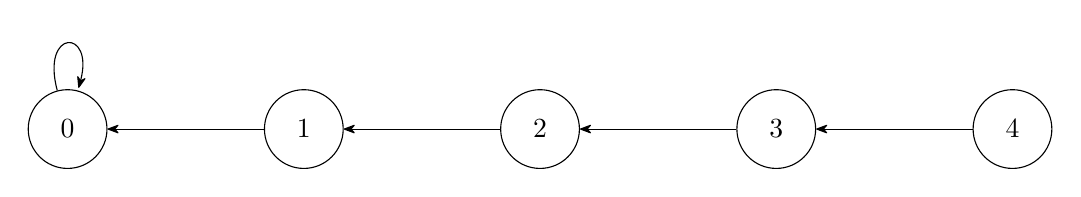
\begin{tikzpicture}[>={Stealth[round]}, node distance=2cm and 1cm, every node/.style={circle, draw, minimum size=1cm}]
    % Define vertices
    \node (v0) at (0, 0) {0};
    \node (v1) at (3, 0) {1};
    \node (v2) at (6, 0) {2};
    \node (v3) at (9, 0) {3};
    \node (v4) at (12, 0) {4};
    
    % Draw edges
    \draw [->] (v1) to (v0); % Edge 1 -> 0
    \draw [->] (v2) to (v1); % Edge 2 -> 1
    \draw [->] (v3) to (v2); % Edge 3 -> 2
    \draw [->] (v4) to (v3); % Edge 4 -> 3
    \draw[->] (v0) edge[loop above] (v0); % Self-loop at 0
\end{tikzpicture}
}
\end{center}
Run the SageMath script \texttt{ex1325.sage} to verify.
\end{example}

\section{The Composition Lemma}

\begin{prop}[Composition Inequality]\label{prop:composition-lemma-ineq}
  %\lean{}
  %\leanok
  %\uses{defn:graceful-functional-graphs, defn:graceful-functional-graphs-set, prop:multivariate-quotient-remainder, defn:polynomial-grace-definition, defn:polynomial-congruence, prop:polynomial-grace-certificate}
Consider an arbitrary $f\in\mathbb{Z}_{n}^{\mathbb{Z}_{n}}$ subject to the fixed point condition
$\left|f^{\left(n-1\right)}\left(\mathbb{Z}_{n}\right)\right|=1$. The following statements are equivalent:
\begin{enumerate}
    \item 
    \[
    \max_{\sigma\in\text{S}_{n}}\big|\{|\sigma f^{(2)}\sigma^{-1}(i)-i|:i\in\mathbb{Z}_{n}\}\big|\le\max_{\sigma\in\text{S}_{n}}\big|\{|\sigma f\sigma^{-1}(i)-i|:i\in\mathbb{Z}_{n}\}\big|.
    \]
    \item
    \[
    P_{f^{(2)}} ({\bf x}) \not\equiv 0  \implies  P_{f} ({\bf x}) \not\equiv 0.
    \]
    \item 
    \[
    \text{GrL}(G_f) \neq \varnothing
    \]
\end{enumerate}    
\end{prop}
\begin{proof}
If $f\in\mathbb{Z}_{n}^{\mathbb{Z}_{n}}$ is identically constant,
then $G_{f}$ is graceful. We see this from the fact that the functional
digraph of the identically zero function is gracefully labeled and the fact that
functional digraphs of identically constant functions are all isomorphic. It follows
that all functional directed graphs having diameter less than $3$ are graceful. Consequently,
all claims hold for all functional digraphs of diameter less than $3$. We now turn our attention
to functional trees of diameter greater or equal to $3$. 
It follows by definition 
\begin{equation}
n=\max_{\sigma\in\text{S}_{n}}\big|\{|\sigma f\sigma^{-1}(i)-i|:i\in\mathbb{Z}_{n}\}\big|\iff P_{f}({\bf x})\not\equiv0\iff\text{GrL}(G_{f})\neq\varnothing.
\end{equation}
We now proceed to show (i) $\iff$ (iii). The backward claim is the simplest of the two claims. We see
that if $f$ is contractive, so too is $f^{(2)}$. Then 
assertions
\begin{equation}
n=\max_{\sigma\in\text{S}_{n}}\big|\{|\sigma f^{(2)}\sigma^{-1}(i)-i|:i\in\mathbb{Z}_{n}\}\big|\text{  and  }n=\max_{\sigma\in\text{S}_{n}}\big|\{|\sigma f\sigma^{-1}(i)-i|:i\in\mathbb{Z}_{n}\}\big|
\end{equation}
indeed implies the inequality
\begin{equation}
\max_{\sigma\in\text{S}_{n}}\big|\{|\sigma f^{(2)}\sigma^{-1}(i)-i|:i\in\mathbb{Z}_{n}\}\big|\le\max_{\sigma\in\text{S}_{n}}\big|\{|\sigma f\sigma^{-1}(i)-i|:i\in\mathbb{Z}_{n}\}\big|.
\end{equation}
We now establish the forward claim by contradiction. Assume for the
sake of establishing a contradiction that for some contractive map
$f\in\mathbb{Z}_{n}^{\mathbb{Z}_{n}}$ we have 
\begin{equation}
n>\max_{\sigma\in\text{S}_{n}}\left|\left\{ |\sigma f^{(2)}\sigma^{-1}(i)-i|:i\in\mathbb{Z}_{n}\right\} \right|,
\end{equation}
for we know by the number of edges being equal to $n$ that it is impossible
 that 
\begin{equation}
n<\max_{\sigma\in\text{S}_{n}}\left|\left\{ |\sigma f^{(2)}\sigma^{-1}(i)-i|:i\in\mathbb{Z}_{n}\right\} \right|.
\end{equation}
Note that the range of $f$ is a proper subset of $\mathbb{Z}_{n}$.
By the premise that $f$ is contractive, it follows that $f^{(\left\lceil 2^{\text{lg}(n-1)}\right\rceil )}$
is identically constant and thus 
\begin{equation}
n=\max_{\sigma\in\text{S}_{n}}\left|\left\{ |\sigma f^{(\left\lceil 2^{\text{lg}(n-1)}\right\rceil )}\sigma^{-1}(i)-i|:i\in\mathbb{Z}_{n}\right\} \right|,
\end{equation}
where lg denotes the logarithm base $2$. Consequently there must
be some integer $0\le\kappa<\text{lg}(n-1)$ such that 
\begin{equation}
\max_{\sigma\in\text{S}_{n}}\left|\left\{ |\sigma f^{(\left\lceil 2^{\kappa}\right\rceil )}\sigma^{-1}(i)-i|:i\in\mathbb{Z}_{n}\right\} \right|>\max_{\sigma\in\text{S}_{n}}\left|\left\{ |\sigma f^{(\left\lceil 2^{\kappa-1}\right\rceil )}\sigma^{-1}(i)-i|:i\in\mathbb{Z}_{n}\right\} \right|.
\end{equation}
This contradicts the assertion of statement (i), thereby
establishing the backward claim. 
The exact same reasoning as above establishes (ii) $\iff$ (iii), for we have
\begin{equation}
        P_{f^{\left(\left\lceil 2^{\text{lg}(n-1)}\right\rceil \right)}} ({\bf x}) \not\equiv 0. 
\end{equation}
\end{proof}

Having assembled together the pieces required to prove our main result, we proceed to fit the pieces together to state and prove the \textit{Composition Lemma}.
\begin{lemma}[Composition Lemma]\label{lem:composition-lemma}
    %\lean{}
  %\leanok
  %\uses{defn:graceful-functional-graphs, defn:graceful-functional-graphs-set, prop:multivariate-quotient-remainder, defn:polynomial-grace-definition, defn:polynomial-congruence, prop:polynomial-grace-certificate, prop:composition-lemma-ineq}
 For all contractive  $f\in\mathbb{Z}_{n}^{\mathbb{Z}_{n}}$, i.e., functions subject to the fixed point condition
$\left|f^{\left(n-1\right)}\left(\mathbb{Z}_{n}\right)\right|=1$,
we have
\begin{equation}\label{eq:composition-lemma}
\max_{\sigma\in\text{S}_{n}}\big|\{|\sigma f^{(2)}\sigma^{-1}(i)-i|:i\in\mathbb{Z}_{n}\}\big|\le\max_{\sigma\in\text{S}_{n}}\big|\{|\sigma f\sigma^{-1}(i)-i|:i\in\mathbb{Z}_{n}\}\big|.
\end{equation}
\end{lemma}
\begin{proof}
Owing to Proposition \ref{prop:composition-lemma-ineq}, we prove the statement by establishing 
\[
    P_{f^{(2)}} ({\bf x}) \not\equiv 0  \implies  P_{f} ({\bf x}) \not\equiv 0.
\]
For simplicity, we prove a generalization of the desired claim. Assume without loss of generality that
\[
f(i)>i,\ \forall\:i\in\mathbb{Z}_{n-1}\text{  and  }f(n-1)=n-1.
\]
Further assume without loss of generality that the vertex labeled $0$ is at furthest edge distance from the root in $G_f$ (i.e. the vertex labeled $n-1$). Given that the diameter of $G_{f}$ is greater than $2$, we may also assume without loss of generality that  $f^{-1}\left(\{0\}\right)=\varnothing$
and $f^{(2)}(0)\ne f(0)$. Let the contractive
map $g\in\mathbb{Z}_{n}^{\mathbb{Z}_{n}}$ be devised from $f$ such that 
\begin{equation}
g(i)=\begin{cases}
\begin{array}{cc}
f^{(2)}(i) & \text{ if }i\in f^{-1}\big(\{f(0)\}\big)\\
f(i) & \text{otherwise}
\end{array},\ \forall\,i\in\mathbb{Z}_{n}.\end{cases}
\end{equation}
We show that
\begin{equation} \label{eq:composition-lemma-generalized}
P_{g} ({\bf x}) \not\equiv 0  \implies  P_{f} ({\bf x}) \not\equiv 0.
\end{equation}
Note that the assertion immediately above generalizes the composition
lemma since, $f$ is only partially
iterated. More precisely, we iterate $f$ on the subset $f^{-1}\big(\{f(0)\}\big)$.
In turn, iterating (at most $n-1$ times) this generalization  of the composition lemma yields
that all functional trees are graceful, which in turn implies that the \textit{Composition Lemma} as stated in Lemma \ref{eq:composition-lemma}  holds. For notational convenience, assume without loss of generality that 
\begin{equation}
f^{-1}\big(\{f(0)\}\big)=\mathbb{Z}_{\left|f^{-1}\big(\{f(0)\}\big)\right|}\text{  and  }f(0)=\left|f^{-1}\big(\{f(0)\}\big)\right|.
\end{equation}
If the conditions stated above are not met, we relabel the vertices of $G_f$ to ensure that such is indeed the case. In the remainder of the proof let $p$ be the smallest prime subject to $2n-1\le p$. We consider the slight variant of the polynomial certificate construction given by
\[
\mathcal{P}_{f}(\mathbf{x})\coloneq\underbrace{\prod_{0\le u<v<n}(x_{v}-x_{u})}_{V(x_{0},\ldots,x_{n-1})}\,\underbrace{\prod_{i\in\mathbb{Z}_{n}}\big(\prod_{j\in\mathbb{Z}_{p}\backslash\mathbb{Z}_{n}}(x_{i}-j)\big)}_{\mathcal{S}(x_{0},\ldots,x_{n-1})}\,\underbrace{\prod_{0\le u<v<n}\bigg(\prod_{t\in\mathbb{Z}_{2}}\big((x_{f(v)}-x_{v})+(-1)^{t}(x_{f(u)}-x_{u})\big)\bigg)}_{E_{f}(x_{0},\ldots,x_{n-1})}.
\]
In which case the canonical representative of the congruence class of $\mathcal{P}_f$ modulo the polynomials ideal generated by members of the set
\[
\bigg\{\prod_{j\in\mathbb{Z}_{p}}(x_{i}-j):i\in\mathbb{Z}_{n}\bigg\}
\]
is given by
\begin{equation} \label{eq:new-graceful-evaluation}
\overline{\mathcal{P}_{f}}(\mathbf{x})=\prod_{v\in\mathbb{Z}_{n}}(v!)^{2}\frac{(n-1+v)!}{(2v)!}\prod_{i\in\mathbb{Z}_{n}}\big(\prod_{j\in\mathbb{Z}_{p}\backslash\mathbb{Z}_{n}}(i-j)\big)\sum_{\begin{array}{c}
\substack{\sigma\in\text{S}_{n}\\
\text{s.t.}\\
\left|\sigma f-\sigma\right|\in\text{S}_{n}
}
\end{array}}\text{sgn}(\sigma\left|\sigma f-\sigma\right|)\prod_{\begin{array}{c}
\substack{i\in\mathbb{Z}_{n}\\
j_{i}\in\mathbb{Z}_{p}\backslash\{\sigma(i)\}
}
\end{array}}\big(\frac{x_{i}-j_{i}}{\sigma(i)-j_{i}}\big),
\end{equation}
which is a polynomial of degree at most $p-1$ in each variable and
\[
\prod_{v\in\mathbb{Z}_{n}}(v!)^{2}\frac{(n-1+v)!}{(2v)!}\prod_{i\in\mathbb{Z}_{n}}\big(\prod_{j\in\mathbb{Z}_{p}\backslash\mathbb{Z}_{n}}(i-j)\big)\not\equiv0\mod p.
\]
A similar expansion holds for $g$, with the same coefficient up to sign. Next, roughly speaking, we show that there exist a in invertible linear transformation which  maps $\mathcal{P}_f$ to $\mathcal{P}_g$ and vice versa. For an arbitrary $h\in \mathbb{Z}_{n}^{\mathbb{Z}_{n}}$ let $A_{h}\in\{0,1\}^{n\times n}$ denote the adjacency matrix of the functional directed graph $G_h$ i.e.
\[
A_{h}[u,v]=\begin{cases}
\begin{array}{cc}
1 & \text{ if }v=h(u)\\
0 & \text{otherwise}
\end{array}, & \forall\,(u,v)\in\mathbb{Z}_{n}\times\mathbb{Z}_{n}\end{cases}.
\]
Observe that signed incidence matrices $(A_{\text{id}}-A_{f})$ and $(A_{\text{id}}-A_{g})$ of $G_f$ and $G_g$ respectively are both in Row-Echelon form. Induced edge label binomials $x_i-x_{f(i)}$ and $x_i-x_{g(i)}$ correspond to the $i$-th entry of $(A_{\text{id}}-A_{f})\cdot \mathbf{x}$ and $(A_{\text{id}}-A_{g})\cdot \mathbf{x}$ respectively. Given that $G_f$ is a functional tree, for each one of the ${n \choose 2}$ vertex pair $(i,\,j)$ where $0\le i < j <n$, there exist a unique $\mathbf{v}_{i,j}\in\{-1,0,1\}^{n\times1}$ such that
\[
(x_{j}-x_{i})=\mathbf{v}_{i,j}^{\top}\cdot (A_{\text{id}}-A_{f})\cdot\mathbf{x}.
\]
By introducing a distinct variable $y_{i,j}$ for each one of the ${n \choose 2}$ vertex pair $(i,\,j)$ where $0\le i < j <n$, we subsequently make use of the equality
\[
y_{i,j}\,(x_{j}-x_{i})=(y_{i,j}\mathbf{v}_{i,j})^{\top}\cdot(A_{\text{id}}-A_{f})\cdot\mathbf{x}.
\]
in expressing the multiple of the vertex Vandermonde factor
\[
\prod_{0\le i<j<n}y_{i,j}\,(x_{j}-x_{i})=\prod_{0\le i<j<n}\big((y_{i,j}\mathbf{v}_{i,j})^{\top}\cdot(A_{\text{id}}-A_{f})\cdot\mathbf{x}\big).
\]
Similarly the absolute induced edge label Vandermonde factor is expressed by
\[
\prod_{0\le u<v<n}\bigg(\prod_{t\in\mathbb{Z}_{2}}\big((x_{f(v)}-x_{v})+(-1)^{t}(x_{f(u)}-x_{u})\big)\bigg)=\prod_{0\le i<j<n}\,\prod_{t\in\mathbb{Z}_{2}}\bigg(\big(A_{\text{id}}[j,:]\cdot(A_{\text{id}}-A_{f})+(-1)^{t}A_{\text{id}}[i,:]\cdot(A_{\text{id}}-A_{f})\big)\cdot\mathbf{x}\bigg).
\]
Let
\[
\mathcal{P}_{f}(\mathbf{x},Y)\coloneq
\]
\[
\prod_{0\le i<j<n}\big((y_{i,j}\mathbf{v}_{i,j})^{\top}\cdot(A_{\text{id}}-A_{f})\cdot\mathbf{x}\big)\,\mathcal{S}(x_{0},\ldots,x_{n-1})\,\prod_{0\le i<j<n}\,\prod_{t\in\mathbb{Z}_{2}}\bigg(\big(A_{\text{id}}[j,:]\cdot(A_{\text{id}}-A_{f})+(-1)^{t}A_{\text{id}}[i,:]\cdot(A_{\text{id}}-A_{f})\big)\cdot\mathbf{x}\bigg).
\]

We bypass ring homomorphisms from $\mathbb{Q}[x_0,\ldots , x_{n-1}]$ to the quotient ring $\nicefrac{\mathbb{Q}[x_{0},\ldots,x_{n-1}]}{\text{Ideal generated by }\big\{\underset{j\in\mathbb{Z}_{p}}{\prod}(x_{i}-j):i\in\mathbb{Z}_{n}\big\}}$ in our analysis by switching the ground field from $\mathbb{Q}$ to the Galois field of order $p$. More precisely we work over the ring $(\nicefrac{\mathbb{Z}}{p\mathbb{Z}})[x_{0},\ldots,x_{n-1}]$ instead of $\mathbb{Q}[x_{0},\ldots,x_{n-1}]$. Over the said ring the polynomial $\mathcal{P}_f(\mathbf{x})$ is indistinguishable from $\overline{\mathcal{P}_{f}}(\mathbf{x})$ in \ref{eq:new-graceful-evaluation}.
In order for variables to be consistently treated by our proposed linear transformation, we re-express the polynomial $\mathcal{P}_{f}(\mathbf{x},Y)$ by replacing the factor $\mathcal{S}(x_{0},\ldots,x_{n-1})$
with an expression featuring instead
\[
\mathcal{S}_{r}(x_{0},\ldots,x_{r-1},x_{r},x_{r+1},\ldots,x_{n-1},Y)\coloneq\prod_{i<r}\bigg(\prod_{j\in\mathbb{Z}_{p}\backslash\mathbb{Z}_{n}}\big(-y_{i,r}\,(x_{r}-x_{i})-j\,y_{i,r}\big)\bigg)\prod_{i>r}\bigg(\prod_{j\in\mathbb{Z}_{p}\backslash\mathbb{Z}_{n}}\big(y_{r,i}\,(x_{i}-x_{r})-j\,y_{r,i}\big)\bigg),
\]
for all $r\in \mathbb{Z}_n$. In other words
\[
\mathcal{S}_{r}(x_{0},\ldots,x_{r-1},x_{r},x_{r+1},\ldots,x_{n-1},Y)=
\]
\[
\prod_{i<r}\bigg(\prod_{j\in\mathbb{Z}_{p}\backslash\mathbb{Z}_{n}}\big(-(y_{i,r}\mathbf{v}_{i,r})^{\top}\cdot(A_{\text{id}}-A_{f})\cdot\left(\begin{array}{c}
x_{0}\\
\vdots\\
x_{r-1}\\
x_{r}\\
x_{r+1}\\
\vdots\\
x_{n-1}
\end{array}\right)-j\,y_{i,r}\big)\bigg)\prod_{i>r}\bigg(\prod_{j\in\mathbb{Z}_{p}\backslash\mathbb{Z}_{n}}\big((y_{r,i}\mathbf{v}_{r,i})^{\top}\cdot(A_{\text{id}}-A_{f})\cdot\left(\begin{array}{c}
x_{0}\\
\vdots\\
x_{r-1}\\
x_{r}\\
x_{r+1}\\
\vdots\\
x_{n-1}
\end{array}\right)-j\,y_{r,i}\big)\bigg)
\]
Over the chosen ring the following equality holds
\[
\mathcal{P}_{f}(\mathbf{x},Y)=\sum_{r\in\mathbb{Z}_{n}}\mathcal{P}_{f}(\left(\begin{array}{c}
x_{0}\\
\vdots\\
x_{r-1}\\
0\\
x_{r+1}\\
\vdots\\
x_{n-1}
\end{array}\right),Y)
\]

\[
\implies \mathcal{P}_{f}(\mathbf{x},Y)=\sum_{r\in\mathbb{Z}_{n}}\prod_{0\le i<j<n}\big((y_{i,j}\mathbf{v}_{i,j})^{\top}\cdot(A_{\text{id}}-A_{f})\cdot\left(\begin{array}{c}
x_{0}\\
\vdots\\
x_{r-1}\\
0\\
x_{r+1}\\
\vdots\\
x_{n-1}
\end{array}\right)\big)\,\mathcal{S}_{r}(x_{0},\ldots,x_{r-1},0,x_{r+1},\ldots,x_{n-1},Y)\,\times
\]
\[
\prod_{0\le i<j<n}\,\prod_{t\in\mathbb{Z}_{2}}\bigg(\big(A_{\text{id}}[j,:]\cdot(A_{\text{id}}-A_{f})+(-1)^{t}A_{\text{id}}[i,:]\cdot(A_{\text{id}}-A_{f})\big)\cdot\left(\begin{array}{c}
x_{0}\\
\vdots\\
x_{r-1}\\
0\\
x_{r+1}\\
\vdots\\
x_{n-1}
\end{array}\right)\bigg).
\]
Thus we have expressed $\mathcal{P}_{f}(\mathbf{x},Y)$ as a polynomial in the entries of $Y$ as well as the ${n \choose 2}$ binomials $x_j-x_i$ where $0\le i<j<n$. Albeit the factor $\mathcal{S}_r$ features binomials $x_r-x_i$ when $i<r$ as well as binomials $x_i-x_r$ when $r<i$ where the variable $x_r$ is evaluated to zero. 

Observe that the set of row linear combinations
\[
\text{Row}_{f(0)}+\text{Row}_{i}\longrightarrow\text{Row}_{i},\ \forall\:i\in f^{-1}\big(\{f(0)\}\big).
\]
converts the incidence matrix $A_{\text{id}}-A_{f}$ to the incidence matrix $A_{\text{id}}-A_{g}$.
These row operations are in turn expressed in terms of left elementary matrix action as follows
\[
\bigg(\prod_{i\in f^{-1}\big(\{f(0)\}\big)}(A_{\text{id}}+A_{\text{id}}[:,i]\cdot A_{\text{id}}[f(0),:])\bigg)\cdot(A_{\text{id}}-A_{f})=(A_{\text{id}}-A_{g}).
\]
Consider the invertible linear transformation which effects simultaneous maps
\[
\mathbf{x}\mapsto\bigg(\prod_{i\in f^{-1}\big(\{f(0)\}\big)}(A_{\text{id}}+A_{\text{id}}[:,i]\cdot A_{\text{id}}[f(0),:])\bigg)\cdot\mathbf{x}\text{ and }y_{i,j}\mathbf{v}_{i,j}^{\top}\mapsto y_{i,j}\mathbf{v}_{i,j}^{\top}\cdot\bigg(\prod_{i\in f^{-1}\big(\{f(0)\}\big)}(A_{\text{id}}-A_{\text{id}}[:,i]\cdot A_{\text{id}}[f(0),:])\bigg).
\]
In other words the vector
\[
\left(\begin{array}{c}
\mathbf{x}\\
y_{0,1}\mathbf{v}_{0,1}\\
\vdots\\
y_{i,j}\mathbf{v}_{i,j}\\
\vdots\\
y_{n-2,n-1}\mathbf{v}_{n-2,n-1}
\end{array}\right)
\]
is mapped to
\[
\left(\big(\prod_{i\in f^{-1}\big(\{f(0)\}\big)}(A_{\text{id}}+A_{\text{id}}[:,i]\cdot A_{\text{id}}[f(0),:])\big)\oplus\bigg(I_{{n \choose 2}}\otimes\big(\prod_{i\in f^{-1}\big(\{f(0)\}\big)}(A_{\text{id}}-A_{\text{id}}[:,i]\cdot A_{\text{id}}[f(0),:])\big)^{\top}\bigg)\right)\cdot\left(\begin{array}{c}
\mathbf{x}\\
y_{0,1}\mathbf{v}_{0,1}\\
\vdots\\
y_{i,j}\mathbf{v}_{i,j}\\
\vdots\\
y_{n-2,n-1}\mathbf{v}_{n-2,n-1}
\end{array}\right).
\]
Thus resulting in a map of $\mathcal{P}_{f}(\mathbf{x},Y)$ to  $\mathcal{P}_{g}(\mathbf{x},Y)$ for all $\mathbf{x}\in(\nicefrac{\mathbb{Z}}{p\mathbb{Z}})^{n\times1}$. If the induced function
\[
\mathcal{P}_{f}(\mathbf{x},Y)=F_{f}(y_{0,1}\mathbf{v}_{0,1},\ldots,y_{i,j}\mathbf{v}_{i,j},\ldots,y_{n-2,n-1}\mathbf{v}_{n-2,n-1})
\]
 vanishes identically in the ring $(\nicefrac{\mathbb{Z}}{p\mathbb{Z}})[y_{0,1},\ldots,y_{n-2,\,n-1}]$ then for all
 \[
 \bigg(\prod_{i\in f^{-1}\big(\{f(0)\}\big)}(A_{\text{id}}+A_{\text{id}}[:,i]\cdot A_{\text{id}}[f(0),:])\bigg)\cdot\mathbf{x}\in(\nicefrac{\mathbb{Z}}{p\mathbb{Z}})^{n\times1},
 \]
 the corresponding induced polynomials also vanishes identically in the ring $(\nicefrac{\mathbb{Z}}{p\mathbb{Z}})[y_{0,1},\ldots,y_{n-2,\,n-1}]$. For we see that
 \[
 \mathcal{P}_{f}(\mathbf{x},Y)=\mathcal{P}_{f}\bigg(\big(\prod_{i\in f^{-1}\big(\{f(0)\}\big)}(A_{\text{id}}+A_{\text{id}}[:,i]\cdot A_{\text{id}}[f(0),:])\big)\cdot\big(\prod_{i\in f^{-1}\big(\{f(0)\}\big)}(A_{\text{id}}+A_{\text{id}}[:,i]\cdot A_{\text{id}}[f(0),:])\big)^{-1}\cdot\mathbf{x},Y\bigg)
 \]
 \[
 =\mathcal{P}_{f}\bigg(\big(\prod_{i\in f^{-1}\big(\{f(0)\}\big)}(A_{\text{id}}+A_{\text{id}}[:,i]\cdot A_{\text{id}}[f(0),:])\big)\cdot\mathbf{x}^{\prime},Y\bigg),
 \]
 where $\mathbf{x}^{\prime}\in(\nicefrac{\mathbb{Z}}{p\mathbb{Z}})^{n\times1}$ in the equality immediately above is such that
 \[
\mathbf{x}^{\prime}=\big(\prod_{i\in f^{-1}\big(\{f(0)\}\big)}(A_{\text{id}}+A_{\text{id}}[:,i]\cdot A_{\text{id}}[f(0),:])\big)^{-1}\cdot\mathbf{x}=\big(\prod_{i\in f^{-1}\big(\{f(0)\}\big)}(A_{\text{id}}-A_{\text{id}}[:,i]\cdot A_{\text{id}}[f(0),:])\big)\cdot\mathbf{x}.
 \]
 Thus the ring isomorphism which maps the induced $F_{f}(y_{0,1}\mathbf{v}_{0,1},\ldots,y_{n-2,n-1}\mathbf{v}_{n-2,n-1})$ in $(\nicefrac{\mathbb{Z}}{p\mathbb{Z}})[y_{0,1},\ldots,y_{n-2,\,n-1}]$ to its image 
 \[
 F_{f}\bigg(\big(\prod_{i\in f^{-1}\big(\{f(0)\}\big)}(A_{\text{id}}-A_{\text{id}}[:,i]\cdot A_{\text{id}}[f(0),:])\big)^{\top}y_{0,1}\mathbf{v}_{0,1},\ldots,\big(\prod_{i\in f^{-1}\big(\{f(0)\}\big)}(A_{\text{id}}-A_{\text{id}}[:,i]\cdot A_{\text{id}}[f(0),:])\big)^{\top}y_{n-2,n-1}\mathbf{v}_{n-2,n-1}\bigg),
 \]
 ensures that the image induced polynomial function of vectors vanish identically if its pre-image vanishes identically for all 
 \[
 \bigg(\prod_{i\in f^{-1}\big(\{f(0)\}\big)}(A_{\text{id}}+A_{\text{id}}[:,i]\cdot A_{\text{id}}[f(0),:])\bigg)\cdot\mathbf{x}\in(\nicefrac{\mathbb{Z}}{p\mathbb{Z}})^{n\times1}.
 \]
 By which if $\mathcal{P}_{g}(\mathbf{x},Y)$ admits a non-vanishing point for some assignment of $\mathbf{x}\in(\nicefrac{\mathbb{Z}}{p\mathbb{Z}})^{n\times1}$ then $\mathcal{P}_{f}(\mathbf{x},Y)$ also admits a non-vanishing point for some assignment of $\mathbf{x}\in(\nicefrac{\mathbb{Z}}{p\mathbb{Z}})^{n\times1}$ which yields in turn that
 \[
 \big(P_{g}(\mathbf{x})\not\equiv0\mod\big\{\underset{j\in\mathbb{Z}_{n}}{\prod}(x_{i}-j):i\in\mathbb{Z}_{n}\big\}\big)\implies\big(P_{f}(\mathbf{x})\not\equiv0\mod\big\{\underset{j\in\mathbb{Z}_{n}}{\prod}(x_{i}-j):i\in\mathbb{Z}_{n}\big\}\big)
 \]
 as claimed.
\end{proof}

\begin{example} The figure below illustrates the local iteration described in the proof of Lemma \ref{lem:composition-lemma} with an example of a path on 5 vertices.
\ \\
\begin{center}   $G_f: \;$
\resizebox{!}{3em}{
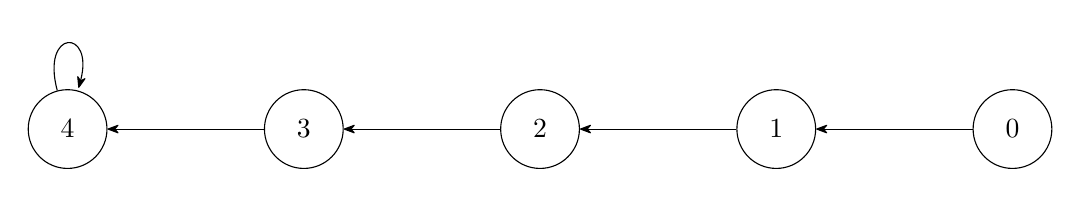
\begin{tikzpicture}[>={Stealth[round]}, node distance=2cm and 1cm, every node/.style={circle, draw, minimum size=1cm}]
    % Define vertices
    \node (v0) at (0, 0) {4};
    \node (v1) at (3, 0) {3};
    \node (v2) at (6, 0) {2};
    \node (v3) at (9, 0) {1};
    \node (v4) at (12, 0) {0};
    
    % Draw edges
    \draw [->] (v1) to (v0); % Edge 1 -> 0
    \draw [->] (v2) to (v1); % Edge 2 -> 1
    \draw [->] (v3) to (v2); % Edge 3 -> 2
    \draw [->] (v4) to (v3); % Edge 4 -> 3
    \draw[->] (v0) edge[loop above] (v0); % Self-loop at 0
\end{tikzpicture}
}
\end{center}
\ \\
\begin{center}   
$G_g: \;$
\resizebox{!}{3em}{
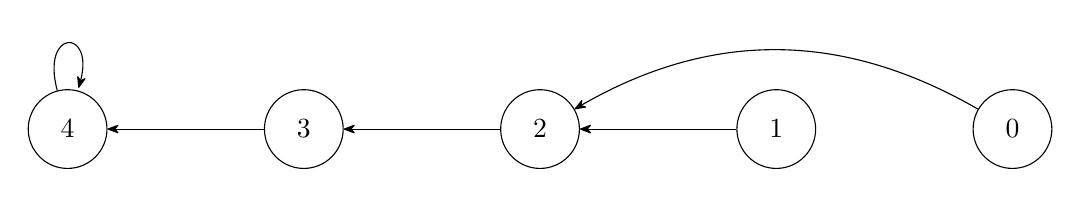
\begin{tikzpicture}[>={Stealth[round]}, node distance=2cm and 1cm, every node/.style={circle, draw, minimum size=1cm}]
    % Define vertices
    \node (v0) at (0, 0) {4};
    \node (v1) at (3, 0) {3};
    \node (v2) at (6, 0) {2};
    \node (v3) at (9, 0) {1};
    \node (v4) at (12, 0) {0};
    
    % Draw edges
    \draw [->] (v1) to (v0); % Edge 1 -> 0
    \draw [->] (v2) to (v1); % Edge 2 -> 1
    \draw [->] (v3) to (v2); % Edge 3 -> 2
    \draw [->] (v4) edge[bend right] (v2); % Edge 4 -> 2
    \draw[->] (v0) edge[loop above] (v0); % Self-loop at 0
\end{tikzpicture}
}
\end{center}
\end{example}


\bibliographystyle{alpha}
\bibliography{biblio}

\end{document}


%\home{https://emilyriehl.github.io/infinity-cosmos}
%\github{https://github.com/emilyriehl/infinity-cosmos}
%\dochome{https://emilyriehl.github.io/infinity-cosmos/docs}

\title{Composition Lemma}
\author{Edinah Gnang}
\author{Parikshit Chalise}

\begin{document}
\linenumbers
\maketitle
\tableofcontents

`% In this file you should put the actual content of the blueprint.
% It will be used both by the web and the print version.
% It should *not* include the \begin{document}
%
% If you want to split the blueprint content into several files then
% the current file can be a simple sequence of \input. Otherwise It
% can start with a \section or \chapter for instance.

\chapter{\texorpdfstring{Composition Lemma}{Composition Lemma}}

\section{Overview}
The \textit{Composition Lemma} was developed and refined over 6 years, beginning in 2018, as a novel approach to settle in the affirmative the \textit{Graceful Tree Conjecture}. The first of such papers was posted in \cite{gnang2020gracefullabelingstrees} by Gnang. A further developed series of papers resolving the same conjecture again appeared in \cite{gnang2022compositionlemma} and \cite{gnang2023proofkotzigringelrosaconjecture}. Recently, the same method has been applied to settle other longstanding conjectures in \cite{chalise2024treenedgesdecomposes} and \cite{chalise2024prooftreepackingconjecture}. We comment that the series of papers shared on the open-source platform arXiv reflect the evolving landscape of Gnang's thought process, and the frequent re-uploads were driven by the natural progression and refinement of ideas. However, we recognize that these numerous edits may have unintentionally caused confusion and raised questions regarding the success of the method. In the current work, we aim to address these concerns by presenting a detailed blueprint of the proof, with the goal of formalizing it in Lean4.

\section{Functional Directed Graphs}\label{sec:Functional Directed Graphs}
For notational convenience, let $\mathbb{Z}_{n}$ denote the set whose members are the smallest $n$ non-negative integers, i.e.,
\begin{equation}
\mathbb{Z}_{n}:=\big\{0,\ldots,\,n-1\big\}.
\end{equation}
For a function $f:\mathbb{Z}_{m}\to\mathbb{Z}_{n}$, we write $f\in\mathbb{Z}_{n}^{\mathbb{Z}_{m}}$.
For $X\subseteq\mathbb{Z}_{m}$, $f(X)$ denotes the image of $X$
under $f$, i.e.,
\begin{equation}
f(X)=\{f(i):i\in X\},
\end{equation}
and $|f(X)|$ denotes its
cardinality. For $Y\subseteq\mathbb{Z}_{n}\ensuremath{,}f^{-1}(Y)$
denotes the pre-image of $Y$ under $f$ i.e.
\begin{equation}
f^{-1}(Y)=\{j\in\mathbb{Z}_{m}:f(j)\in Y\}
\end{equation}
\begin{definition}[Functional digraphs]\label{defn:functional-directed-graphs}
% REVIEW THE LEAN LABELS BELLOW:
  %\lean{}
  %\leanok
  %\uses{defn:standard-simplex}
For an arbitrary $f\in \mathbb{Z}_n^{\mathbb{Z}_n}$, the \emph{functional directed graph} prescribed by $f$, denoted $G_f$, is such that the vertex set $V(G_f)$ and the directed edge set $E(G_f)$ are respectively as follows:
\[
V(G_f) = \mathbb{Z}_n, \; E(G_f) = \{(v,f(v)):v \in \mathbb{Z}_n\}.
\]
\end{definition}
\begin{definition}[Graceful functional digraphs]\label{defn:graceful-functional-graphs}
  %\lean{}
  %\leanok
  %\uses{defn:functional-directed-graphs}
The functional directed graph prescribed by $f\in\mathbb{Z}_{n}^{\mathbb{Z}_{n}}$ is graceful if there exist
a bijection $\sigma\in \text{S}_n \subset
 \mathbb{Z}_{n}^{\mathbb{Z}_{n}}$ such that
\begin{equation}
\big\{\left|\sigma f\sigma^{-1}(i)-i\right|:i\in\mathbb{Z}_{n}\big\}=\mathbb{Z}_{n}.
\end{equation}
If $\sigma=\text{id}$ (the identity function), then $G_{f}$ --- the functional directed graph prescribed by $f$ --- is gracefully labeled. 
\end{definition}
\begin{defn}[Automorphism group]\label{defn:aut-functional-graphs}
  %\lean{}
  %\leanok
  %\uses{defn:functional-directed-graphs}
For a functional directed graph $G_f$, its automorphism group, denoted $\text{Aut}\left(G_f\right)$, is defined as follows:
\[
\text{Aut}(G_{f})=\big\{\sigma\in\text{S}_{n}:\{\big(i,f(i)\big):i\in\mathbb{Z}_{n}\}=\{\big(j,\sigma f\sigma^{-1}(j)\big):j\in\mathbb{Z}_{n}\}\big\}.
\]
For a polynomial $P \in \mathbb{C}[x_0, \ldots, x_{n-1}]$, its automorphism group, is the stablizer of $P$ and denoted $\text{Aut($P$)}$. Formally defined as follows:
\[
\text{Aut}\left(P\right)=\large\{\sigma\in\text{S}_{n}:P\left(x_{0},\ldots,x_{i},\ldots,x_{n-1}\right)=P\left(x_{\sigma(0)},\ldots,x_{\sigma(i)},\ldots,x_{\sigma(n-1)}\right)\large\}.
\]
\end{defn}
\begin{definition}[Graceful re-labelings]\label{defn:graceful-functional-graphs-set}
  %\lean{}
  %\leanok
  %\uses{defn:functional-directed-graphs, defn:graceful-functional-graphs}
The set of distinct gracefully labeled functional directed graphs isomorphic to $G_{f}$ is 
\[
\text{GrL}\left(G_{f}\right)\,:=\left\{ G_{\sigma f\sigma^{-1}}:\begin{array}{c}
\sigma\text{ is a representative of a coset in }\nicefrac{\text{S}_{n}}{\text{Aut}\left(G_{f}\right)}\text{ and }\\
\mathbb{Z}_{n}=\left\{ \left|\sigma f\sigma^{-1}\left(i\right)-i\right|\,:\,i\in\mathbb{Z}_{n}\right\} 
\end{array}\right\} 
\]
\end{definition}
\begin{definition}[Complementary labeling involution]\label{defn:complementary-labeling-symmetry}
  %\lean{}
  %\leanok
  %\uses{defn:functional-directed-graphs, defn:graceful-functional-graphs}
If $\varphi=n-1-\text{id}$, i.e. $\varphi \in \mathbb{Z}_{n}^{\mathbb{Z}_{n}}$ such that
\[
\varphi(i)=n-1-i,\, \forall \,i\in \mathbb{Z}_{n},
\]
The complementary labeling involution is defined as the map whose domain and codomain is $\mathbb{Z}_{n}^{\mathbb{Z}_{n}}$ and is prescribed by
\[
f \mapsto \varphi f \varphi^{-1},
\]
for an arbitrary $f\in\mathbb{Z}_{n}^{\mathbb{Z}_{n}}$.
\end{definition}
Observe that for all $f\in \mathbb{Z}_{n}^{\mathbb{Z}_{n}}$ the complementary labeling involution fixes the induced edge label of each edge as seen from the equality
\begin{equation}
\left|f(i)-i\right|=\left|\varphi f(i)-\varphi(i)\right|,\quad\forall\,i\in\mathbb{Z}_{n}.
\end{equation}
In other words, induced edge labels are fixed by the vertex relabeling effected by $\varphi$. We call this induced edge label symmetry the \emph{complementary labeling symmetry} of the functional directed graph $G_f$.

\section{Quotient-Remainder Theorem and Lagrange Interpolation}\label{sec:QRT}
 \begin{proposition}[Multivariate Quotient-Remainder]\label{prop:multivariate-quotient-remainder}
  %\lean{Algebra.Polynomial.FieldDivision}
  %\leanok
  %\uses{}
Let $d(x)\in\mathbb{C}[x]$ be a degree $n$ monic polynomial with
simple roots, i.e.,
\begin{equation}
d(x)=\prod_{i\in\mathbb{Z}_{n}}(x-\alpha_{i})\;\text{ and }\:0\ne\prod_{0\le u<v<n}(\alpha_{v}-\alpha_{u}),
\end{equation}
where $\{\alpha_{u}:u\in\mathbb{Z}_{n}\}\subset\mathbb{C}$. 
For
all $P\in\mathbb{C}[x_{0},\ldots,x_{m-1}]$, there exists a unique remainder
$r(x_{0},\ldots,x_{m-1})\in\mathbb{C}[x_{0},\ldots,x_{m-1}]$ of degree
at most $n-1$ in each variable such that for quotients: $\big\{ q_{k}(x_{0},\ldots,x_{n-1}):k\in\mathbb{Z}_{n}\big\}\subset\mathbb{C}[x_{0},\ldots,x_{n-1}]$, we have
\begin{equation}
P(x_{0},\ldots,x_{m-1})= r(x_{0},\ldots,x_{m-1})+\sum_{u\in\mathbb{Z}_{m}}q_{u}(x_{0},\ldots,x_{m-1})\,d(x_{u}).
\end{equation}
 \end{proposition}
\begin{proof}
  %\leanok
We prove by induction on the number of variables that the remainder admits the expansion
\begin{equation}
r(x_{0},\ldots,x_{m-1})=\sum_{g\in\mathbb{Z}_{n}^{\mathbb{Z}_{m}}}P(\boldsymbol{\alpha}_{g})\prod_{i\in\mathbb{Z}_{m}}\left(\prod_{j_{i}\in\mathbb{Z}_{n}\backslash\{g(i)\}}\bigg(\frac{x_{i}-\alpha_{j_{i}}}{\alpha_{g(i)}-\alpha_{j_{i}}}\bigg)\right),
\end{equation}
where for notational convenience $P(\alpha_{g}):=P(\alpha_{g(0)},\ldots,\alpha_{g(m-1)})$.
The base case stems from the univariate quotient-remainder theorem over the field $\mathbb{C}$. The univariate-quotient remainder theorem over the field $\mathbb{C}$ asserts that there exist
a unique quotient-remainder pair $\big(q(x_{0}),\,r(x_{0})\big)\in\mathbb{C}[x_{0}]\times\mathbb{C}[x_{0}]$
subject to
\begin{equation}
H(x_{0})=q(x_{0})\,d(x_{0})+r(x_{0}),
\end{equation}
where $r(x_{0})\in\mathbb{C}[x_{0}]$ is of degree at most $n-1$.
It is completely determined by its evaluation over $\{\alpha_{i}:i\in\mathbb{Z}_{n}\}$,
and by Lagrange interpolation we have 
\begin{equation}
r(x_{0})=\sum_{g\in\mathbb{Z}_{n}^{\mathbb{Z}_{1}}}H(\alpha_{g(0)})\prod_{j_{0}\in\mathbb{Z}_{n}\backslash\{g(0)\}}\bigg(\frac{x_{0}-\alpha_{j_{0}}}{\alpha_{g(0)}-\alpha_{j_{0}}}\bigg),
\end{equation}
thus establishing the claim in the base case. For the induction step,
assume as our induction hypothesis that for all $F\in\mathbb{C}\left[x_{0},\ldots,x_{m-1}\right]$,
we have
\begin{equation}
F=\sum_{k\in\mathbb{Z}_{m}}q_{k}(x_{0},\ldots,x_{m-1})\,d(x_{k})+\sum_{g\in\mathbb{Z}_{n}^{\mathbb{Z}_{m}}}F(\alpha_{g})\prod_{i\in\mathbb{Z}_{m}}\left(\prod_{j_{i}\in\mathbb{Z}_{n}\backslash\left\{ g(i)\right\} }\left(\frac{x_{i}-\alpha_{j_{i}}}{\alpha_{g(i)}-\alpha_{j_{i}}}\right)\right).
\end{equation}
We proceed to show that the hypothesis implies that every polynomial in
$m+1$ variables also admits a similar expansion, thus establishing
the desired claim. Consider a polynomial $H \in \mathbb{C}[x_{0},\ldots,x_{m}]$. We view $H$ as a univariate polynomial in the variable $x_{m}$ whose coefficients lie in the field of fraction $\mathbb{C}(x_{0},\ldots,x_{m-1})$.
The univariate quotient-remainder theorem over the field of fractions $\mathbb{C}(x_{0},\ldots,x_{m-1})$ asserts that
there exit a unique quotient-remainder pair
\[
\big(q(x_{m}),\,r(x_{m})\big)\in\big(\mathbb{C}(x_{0},\ldots,x_{m-1})\big)[x_{m}]\times\big(\mathbb{C}(x_{0},\ldots,x_{m-1})\big)[x_{m}]
\]
subject to
\begin{equation}
H\big(x_{0},\ldots,x_{m}\big)=q(x_{0},\ldots,x_{m})\,d(x_{m})+r(x_{0},\ldots,x_{m}),
\end{equation}
where $r\left(x_{0},\ldots,x_{m}\right)\in\big(\mathbb{C}(x_{0},\ldots,x_{m-1})\big)[x_{m}]$
is of degree at most $n-1$ in the variable $x_{m}$. We write 
\begin{equation}
r\left(x_{0},\ldots,x_{m}\right)=\sum_{k\in\mathbb{Z}_{n}}a_{k}\left(x_{0},\ldots,x_{m-1}\right)\,(x_{m})^{k}.
\end{equation}
We now show that coefficients $\big\{ a_k(x_{0},\ldots,x_{m-1}):k\in \mathbb{Z}_n \big\}$ all lie in the polynomial ring $\mathbb{C}[x_{0},\ldots,x_{m-1}]$
via the equality 
\begin{equation}
\bigg(\text{Vander}\left(\begin{array}{c}
\alpha_{0}\\
\vdots\\
\alpha_{u}\\
\vdots\\
\alpha_{n-1}
\end{array}\right)\bigg)\cdot\left(\begin{array}{c}
a_{0}\left(x_{0},\ldots,x_{m-1}\right)\\
\vdots\\
a_{u}\left(x_{0},\ldots,x_{m-1}\right)\\
\vdots\\
a_{n-1}\left(x_{0},\ldots,x_{m-1}\right)
\end{array}\right)=\left(\begin{array}{c}
H(x_{0},\ldots,x_{m-1},\alpha_{0})\\
\vdots\\
H(x_{0},\ldots,x_{m-1},\alpha_{u})\\
\vdots\\
H(x_{0},\ldots,x_{m-1},\alpha_{n-1})
\end{array}\right),
\end{equation}
where 
\begin{equation}
\bigg(\text{Vander}\left(\begin{array}{c}
\alpha_{0}\\
\vdots\\
\alpha_{u}\\
\vdots\\
\alpha_{u}
\end{array}\right)\bigg)\left[i,j\right]=(\alpha_{i})^{j},\ \forall\,0\le i,j<n.
\end{equation}
Since the Vandermonde matrix is invertible by the fact
\begin{equation}
0\ne\det\bigg(\text{Vander}\left(\begin{array}{c}
\alpha_{0}\\
\vdots\\
\alpha_{u}\\
\vdots\\
\alpha_{u}
\end{array}\right)\bigg)=\prod_{0\le u<v<n}(\alpha_{v}-\alpha_{u}),
 \end{equation}
we indeed have 
\begin{equation}
\left(\begin{array}{c}
a_{0}\left(x_{0},\ldots,x_{m-1}\right)\\
\vdots\\
a_{u}\left(x_{0},\ldots,x_{m-1}\right)\\
\vdots\\
a_{n-1}\left(x_{0},\ldots,x_{m-1}\right)
\end{array}\right)=\bigg(\text{Vander}\left(\begin{array}{c}
\alpha_{0}\\
\vdots\\
\alpha_{u}\\
\vdots\\
\alpha_{u}
\end{array}\right)\bigg)^{-1}\cdot\left(\begin{array}{c}
H(x_{0},\ldots,x_{m-1},\alpha_{0})\\
\vdots\\
H(x_{0},\ldots,x_{m-1},\alpha_{u})\\
\vdots\\
H(x_{0},\ldots,x_{m-1},\alpha_{n-1})
\end{array}\right).
\end{equation}
Therefore, we have 
\begin{equation}
H\big(x_{0},\ldots,x_{m}\big)
= q_{m}\big(x_{0},\ldots,x_{m}\big)\,d(x_{m})+\sum_{g(m)\in\mathbb{Z}_{n}}H\big(x_{0},\ldots,x_{m-1},\alpha_{g(m)}\big)\prod_{j\in\mathbb{Z}_{n}\backslash\{g(m)\}}\left(\frac{x_{m}-\alpha_{j_{m}}}{\alpha_{g(m)}-\alpha_{j_{m}}}\right).
\end{equation}
Applying the induction hypothesis to coefficients
\[
\left\{ H\left(x_{0},\ldots,x_{m-1},\alpha_{g\left(m\right)}\right): \alpha_{g\left(m\right)}\in\mathbb{C}\right\} \subset\mathbb{C}[x_{0},\ldots,x_{m-1}]
\]
yields the desired expansion. Finally, quotients $\big\{ q_{k}(x_{0},\ldots,x_{m-1}):k\in\mathbb{Z}_{m}\big\}$ lie in the polynomial ring $\mathbb{C}[x_{0},\ldots,x_{m-1}]$ since the polynomial $H(x_0,\ldots,x_{m-1})-r(x_0,\ldots,x_{m-1})$ lies in the ideal generated by members of the set $\big\{ d(x_{u}):u\in\mathbb{Z}_{m}\big\}$.
\end{proof}
\begin{proposition}[Ring Homomorphism]\label{prop:ring-homomorphism}
  %\lean{Algebra.Polynomial.FieldDivision}
  %\leanok
  %\uses{}
For an arbitrary $H\in\mathbb{C}\left[x_{0},\ldots,x_{n-1}\right]$, let $\overline{H}$ denote
the {remainder} of the congruence class 
\[
H\text{ modulo the ideal generated by }\left\{ d(x_{i}):i\in\mathbb{Z}_{n}\right\} ,
\]
where
\[
d(x)=\prod_{i\in\mathbb{Z}_{n}}(x-\alpha_{i})\;\text{ and }\:0\ne\prod_{0\le u<v<n}(\alpha_{v}-\alpha_{u}),
\]
Then the following hold:
\begin{enumerate}
    \item For all $g\in\mathbb{Z}_{n}^{\mathbb{Z}_{n}}$, we have $\overline{H}(\boldsymbol{\alpha}_g)=H(\boldsymbol{\alpha}_g)$. 
    \item If $H = H_0 + H_1,$ where $H_0, H_1 \in \mathbb{C}\left[x_{0},\ldots,x_{n-1}\right]$, then $\overline{H_0} + \overline{H_1} = \overline{H}$.
    \item If $H = H_0 \cdot H_1,$ where $H_0, H_1 \in \mathbb{C}\left[x_{0},\ldots,x_{n-1}\right]$,  then $ \overline{H} \equiv \overline{H_0} \cdot \overline{H_1}$.
\end{enumerate}
 \end{proposition}
\begin{proof}
  %\leanok
  The first claim follows from Proposition \ref{prop:multivariate-quotient-remainder} for we see that the divisor vanishes over the lattice. To prove the second claim we recall that
  \[
\overline{H}=\sum_{g\in\mathbb{Z}_{n}^{\mathbb{Z}_{n}}}H(\boldsymbol{\alpha}_{g})\prod_{i\in\mathbb{Z}_{n}}\left(\prod_{j_{i}\in\mathbb{Z}_{n}\backslash\{g(i)\}}\bigg(\frac{x_{i}-\alpha_{j_{i}}}{\alpha_{g(i)}-\alpha_{j_{i}}}\bigg)\right),
  \]
  \[
  \implies\overline{H}=\sum_{g\in\mathbb{Z}_{n}^{\mathbb{Z}_{n}}}\big(H_{0}(\boldsymbol{\alpha}_{g})+H_{1}(\boldsymbol{\alpha}_{g})\big)\prod_{i\in\mathbb{Z}_{n}}\left(\prod_{j_{i}\in\mathbb{Z}_{n}\backslash\{g(i)\}}\bigg(\frac{x_{i}-\alpha_{j_{i}}}{\alpha_{g(i)}-\alpha_{j_{i}}}\bigg)\right),
  \]
  \[
  \implies\overline{H}=\sum_{k\in\mathbb{Z}_{2}}\sum_{g\in\mathbb{Z}_{n}^{\mathbb{Z}_{n}}}H_{k}(\boldsymbol{\alpha}_{g})\prod_{i\in\mathbb{Z}_{n}}\left(\prod_{j_{i}\in\mathbb{Z}_{n}\backslash\{g(i)\}}\bigg(\frac{x_{i}-\alpha_{j_{i}}}{\alpha_{g(i)}-\alpha_{j_{i}}}\bigg)\right).
  \]
  Thus $\overline{H_0} + \overline{H_1} = \overline{H}$ as claimed. Finally the fact (iii) is a straightforward consequence of Proposition \ref{prop:Orthogonality}, which is proved next.
\end{proof}
\begin{proposition}
 \label{prop:Orthogonality}
  %\lean{}
  %\leanok
  %\uses{prop:multivariate-quotient-remainder}   
 Let $f,g \in\mathbb{Z}_{n}^{\mathbb{Z}_{n}}$. For congruence classes prescribed modulo the ideal generated by $\{d(x_{i}):i \in \Z_n\}$, if
\[
d(x)=\prod_{i\in\mathbb{Z}_{n}}(x-\alpha_{i})\;\text{ such that }\:0\ne\prod_{0\le u<v<n}(\alpha_{v}-\alpha_{u}),
\]
then
\[
L_{f}({\bf x})\cdot L_{g}({\bf x})\equiv\begin{cases}
L_{f}({\bf x}) & \text{if }f=g\\
0 & \text{otherwise,}
\end{cases}
\]
\end{proposition}
\begin{proof} Observe that
\[
L_{f}(\mathbf{x})\cdot L_{g}(\mathbf{x})\;=\;\prod_{i\in\mathbb{Z}_{n}}\bigg(\big(c_{i,f}\frac{d(x_{i})}{x_{i}-\alpha_{f(i)}}\big)\big(c_{i,g}\frac{d(x_{i})}{x_{i}-\alpha_{g(i)}}\big)\bigg),
\]
where
\[
c_{i,f}=\prod_{j_{i}\in\mathbb{Z}_{n}\backslash\{f(i)\}}\big(\alpha_{f(i)}-\alpha_{j_{i}}\big)^{-1}\quad\text{ and }\quad c_{i,g}=\prod_{j_{i}\in\mathbb{Z}_{n}\backslash\{g(i)\}}\big(\alpha_{g(i)}-\alpha_{j_{i}}\big)^{-1}.
\]
If $f \neq g$, then there exists $j \in \Z_n$ such that $f(j)\neq g(j)$ and $L_{f}(\mathbf{x})\cdot L_{g}(\mathbf{x})$ is a multiple of $d(x_{j})$,
as a result of which we obtain $L_{f}(\mathbf{x})\cdot L_{g}(\mathbf{x}) \equiv 0$. Alternatively if $f = g$, then
\[
L_{f}(\mathbf{x})\cdot L_{g}(\mathbf{x})=\big(L_{f}(\mathbf{x})\big)^{2}=L_{f}(\mathbf{x})+\bigg(\big(L_{f}(\mathbf{x})\big)^{2}-L_{f}(\mathbf{x})\bigg).
\]
We now show that $\big(L_{f}(\mathbf{x})\big)^{2}-L_{f}(\mathbf{x})\equiv 0$ modulo the ideal generated by $\left\{ d(x_{i}):i\in\mathbb{Z}_{n}\right\}$.
\begin{align*}
\big(L_{f}(\mathbf{x})\big)^{2}-L_{f}(\mathbf{x})\; & =\;L_{f}(\mathbf{x})\left(L_{f}(\mathbf{x})-1\right)\\
 & =\;L_{f}(\mathbf{x})\bigg(L_{f}(\mathbf{x})-\sum_{g\in\mathbb{Z}_{n}^{\mathbb{Z}_{n}}}L_{g}\left({\bf x}\right)\bigg)\\
 & =\;-L_{f}(\mathbf{x})\bigg(\sum_{g\in\mathbb{Z}_{n}^{\mathbb{Z}_{n}}\setminus\{f\}}L_{g}\left({\bf x}\right)\bigg)\\
 & \equiv\;0,
\end{align*}
where the latter congruence identity stems from the prior setting where $f\ne g$.
\end{proof}

\begin{defn}[Polynomial of Grace]\label{defn:polynomial-grace-definition} We define $P_f \in \mathbb{C}[x_0, \ldots, x_{n-1}]$ for all $f \in \mathbb{Z}_n^{\mathbb{Z}_n}$ as follows:
\begin{equation}
    P_f(\mathbf{x}) \coloneq \underbrace{\prod_{0\le u<v<n}(x_{v}-x_{u})}_{V(x_0,\ldots,x_{n-1})}\,\underbrace{\prod_{0\le u<v<n}\big((x_{f(v)}-x_{v})^{2}-(x_{f(u)}-x_{u})^{2}\big)}_{E_f(x_0,\ldots,x_{n-1})}.
\end{equation}
\end{defn}
\begin{defn}[Congruence class]\label{defn:polynomial-congruence}
  %\lean{}  %\leanok
  %\uses{prop:multivariate-quotient-remainder}
For polynomials $P,Q \in \mathbb{C}[x_0, \ldots, x_{n-1}]$, if
\begin{equation}
P({\bf x}) \equiv \; Q({\bf x}) \; \mod\bigg\{\prod_{j\in\mathbb{Z}_{n}}(x_{i}-j):i\in\mathbb{Z}_{n}\bigg\},
\end{equation}
we simply write $P \equiv Q$.
\end{defn}
 Unless otherwise stated, all subsequent congruence identities are prescribed modulo the ideal of polynomials generated by members of the set
\[
\bigg\{\prod_{j\in\mathbb{Z}_{n}}(x_{i}-j):i\in\mathbb{Z}_{n}\bigg\}
\]
\begin{proposition}[Certificate of Grace]\label{prop:polynomial-grace-certificate}
  %\lean{}
  %\leanok
  %\uses{defn:polynomial-grace-definition, defn:polynomial-congruence, prop:multivariate-quotient-remainder}
Let $f\in\mathbb{Z}_{n}^{\mathbb{Z}_{n}}$. The functional
directed graph $G_f$ prescribed by $f$ is graceful if and only if $P_f(\mathbf{x}) \; \not\equiv \; 0$.
\end{proposition}
\begin{proof}
Observe that the vertex Vandermonde factor $V(\mathbf{x})$ is of degree exactly $n-1$ in each variable and therefore equal
to its remainder, i.e.,
\begin{equation}\label{eq:Vf}
V(\mathbf{x})=\sum_{\theta\in\text{S}_{n}}\text{sgn}(\theta)\prod_{i\in\mathbb{Z}_{n}}(x_{i})^{\theta(i)}=\prod_{v\in\mathbb{Z}_{n}}(v!)\;\sum_{\theta\in\text{S}_{n}}\text{sgn}(\theta)\prod_{\begin{array}{c}
\substack{i\in\mathbb{Z}_{n}\\
j_{i}\in\mathbb{Z}_{n}\backslash\{\theta(i)\}
}
\end{array}}\left(\frac{x_{i}-j_{i}}{\theta(i)-j_{i}}\right),
\end{equation}
where 
\begin{equation}
\text{sgn}(\theta):=\prod_{0\le u<v<n}\left(\frac{\theta(v)-\theta(u)}{v-u}\right),\quad\forall\,\theta\in\text{S}_{n}.
\end{equation}
When $n>2$, for every $f\in\mathbb{Z}_{n}^{\mathbb{Z}_{n}}$, the induced edge label Vandermonde factor $E_f(\mathbf{x})$
is of degree $>(n-1)$ in some of its variables. Therefore, by Proposition  \ref{prop:multivariate-quotient-remainder}, we have
\begin{equation}\label{eq:Ef}
E_{f}(\mathbf{x})=\sum_{l\in\mathbb{Z}_{m}}q_{l}(\mathbf{x})\prod_{k\in\mathbb{Z}_{n}}(x_{l}-k)+\prod_{v\in\mathbb{Z}_{n}}(v!)\frac{(n-1+v)!}{(2v)!}\sum_{\begin{array}{c}
g\in\mathbb{Z}_{n}^{\mathbb{Z}_{n}}\\
|gf-g|\in\text{S}_{n}
\end{array}}\text{sgn}(|gf-g|)\prod_{\begin{array}{c}
\substack{i\in\mathbb{Z}_{n}\\
j_{i}\in\mathbb{Z}_{n}\backslash\{g(i)\}
}
\end{array}}\big(\frac{x_{i}-j_{i}}{g(i)-j_{i}}\big).
\end{equation}
Observe that by the expansions in \ref{eq:Vf} and \ref{eq:Ef}, 
\[
P_{f}(\mathbf{x})=\sum_{l\in\mathbb{Z}_{m}}q_{l}(\mathbf{x})V(\mathbf{x})\prod_{k\in\mathbb{Z}_{n}}(x_{l}-k)+
\]
\[
\bigg(\prod_{v\in\mathbb{Z}_{n}}v!\sum_{\theta\in\text{S}_{n}}\text{sgn}(\theta)\prod_{\begin{array}{c}
\substack{i\in\mathbb{Z}_{n}\\
j_{i}\in\mathbb{Z}_{n}\backslash\{\theta(i)\}
}
\end{array}}\big(\frac{x_{i}-j_{i}}{\theta(i)-j_{i}}\big)\bigg)\bigg(\prod_{v\in\mathbb{Z}_{n}}(v!)\frac{(n-1+v)!}{(2v)!}\sum_{\begin{array}{c}
g\in\mathbb{Z}_{n}^{\mathbb{Z}_{n}}\\
|gf-g|\in\text{S}_{n}
\end{array}}\text{sgn}(|gf-g|)\prod_{\begin{array}{c}
\substack{i\in\mathbb{Z}_{n}\\
j_{i}\in\mathbb{Z}_{n}\backslash\{g(i)\}
}
\end{array}}\big(\frac{x_{i}-j_{i}}{g(i)-j_{i}}\big)\bigg).
\]
is congruent to
\begin{equation} \label{eq:graceful-evaluation}
\prod_{v\in\mathbb{Z}_{n}}(v!)^{2}\frac{(n-1+v)!}{(2v)!}\sum_{\begin{array}{c}
\substack{\sigma\in\text{S}_{n}\\
\text{s.t.}\\
\left|\sigma f-\sigma\right|\in\text{S}_{n}
}
\end{array}}\text{sgn}(\sigma\left|\sigma f-\sigma\right|)\prod_{\begin{array}{c}
\substack{i\in\mathbb{Z}_{n}\\
j_{i}\in\mathbb{Z}_{n}\backslash\{\sigma(i)\}
}
\end{array}}\big(\frac{x_{i}-j_{i}}{\sigma(i)-j_{i}}\big),
\end{equation}
where the permutation $|\sigma f-\sigma |$ denotes the induced edge label permutation associated with a graceful relabeling $G_{\sigma f\sigma^{-1}}$ of $G_f$.
The congruence above stems from Prop. \ref{prop:Orthogonality}. A graceful labeling necessitates the integer coefficient
\[
\prod_{0\le i<j<n}(j-i)\big(j^{2}-i^{2})=\prod_{0\le i<j<n}(j-i)^{2}(j+i)=\prod_{v\in\mathbb{Z}_{n}}\left(v!\right)^{2}\frac{\left(n-1+v\right)!}{\left(2v\right)!} \neq 0,
\]
thus establishing the desired claim.
\end{proof}
\begin{example} We present an example of a path on 5 vertices. This is known to be graceful, so we expect a non-zero remainder.
\ \\
\begin{center}   
\resizebox{!}{3em}{
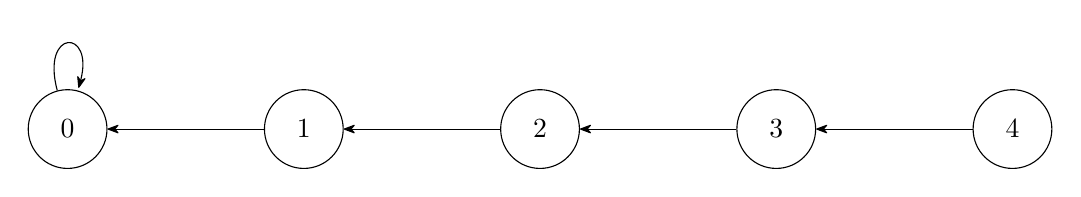
\begin{tikzpicture}[>={Stealth[round]}, node distance=2cm and 1cm, every node/.style={circle, draw, minimum size=1cm}]
    % Define vertices
    \node (v0) at (0, 0) {0};
    \node (v1) at (3, 0) {1};
    \node (v2) at (6, 0) {2};
    \node (v3) at (9, 0) {3};
    \node (v4) at (12, 0) {4};
    
    % Draw edges
    \draw [->] (v1) to (v0); % Edge 1 -> 0
    \draw [->] (v2) to (v1); % Edge 2 -> 1
    \draw [->] (v3) to (v2); % Edge 3 -> 2
    \draw [->] (v4) to (v3); % Edge 4 -> 3
    \draw[->] (v0) edge[loop above] (v0); % Self-loop at 0
\end{tikzpicture}
}
\end{center}
Run the SageMath script \texttt{ex1325.sage} to verify.
\end{example}

\section{The Composition Lemma}

\begin{prop}[Composition Inequality]\label{prop:composition-lemma-ineq}
  %\lean{}
  %\leanok
  %\uses{defn:graceful-functional-graphs, defn:graceful-functional-graphs-set, prop:multivariate-quotient-remainder, defn:polynomial-grace-definition, defn:polynomial-congruence, prop:polynomial-grace-certificate}
Consider an arbitrary $f\in\mathbb{Z}_{n}^{\mathbb{Z}_{n}}$ subject to the fixed point condition
$\left|f^{\left(n-1\right)}\left(\mathbb{Z}_{n}\right)\right|=1$. The following statements are equivalent:
\begin{enumerate}
    \item 
    \[
    \max_{\sigma\in\text{S}_{n}}\big|\{|\sigma f^{(2)}\sigma^{-1}(i)-i|:i\in\mathbb{Z}_{n}\}\big|\le\max_{\sigma\in\text{S}_{n}}\big|\{|\sigma f\sigma^{-1}(i)-i|:i\in\mathbb{Z}_{n}\}\big|.
    \]
    \item
    \[
    P_{f^{(2)}} ({\bf x}) \not\equiv 0  \implies  P_{f} ({\bf x}) \not\equiv 0.
    \]
    \item 
    \[
    \text{GrL}(G_f) \neq \varnothing
    \]
\end{enumerate}    
\end{prop}
\begin{proof}
If $f\in\mathbb{Z}_{n}^{\mathbb{Z}_{n}}$ is identically constant,
then $G_{f}$ is graceful. We see this from the fact that the functional
digraph of the identically zero function is gracefully labeled and the fact that
functional digraphs of identically constant functions are all isomorphic. It follows
that all functional directed graphs having diameter less than $3$ are graceful. Consequently,
all claims hold for all functional digraphs of diameter less than $3$. We now turn our attention
to functional trees of diameter greater or equal to $3$. 
It follows by definition 
\begin{equation}
n=\max_{\sigma\in\text{S}_{n}}\big|\{|\sigma f\sigma^{-1}(i)-i|:i\in\mathbb{Z}_{n}\}\big|\iff P_{f}({\bf x})\not\equiv0\iff\text{GrL}(G_{f})\neq\varnothing.
\end{equation}
We now proceed to show (i) $\iff$ (iii). The backward claim is the simplest of the two claims. We see
that if $f$ is contractive, so too is $f^{(2)}$. Then 
assertions
\begin{equation}
n=\max_{\sigma\in\text{S}_{n}}\big|\{|\sigma f^{(2)}\sigma^{-1}(i)-i|:i\in\mathbb{Z}_{n}\}\big|\text{  and  }n=\max_{\sigma\in\text{S}_{n}}\big|\{|\sigma f\sigma^{-1}(i)-i|:i\in\mathbb{Z}_{n}\}\big|
\end{equation}
indeed implies the inequality
\begin{equation}
\max_{\sigma\in\text{S}_{n}}\big|\{|\sigma f^{(2)}\sigma^{-1}(i)-i|:i\in\mathbb{Z}_{n}\}\big|\le\max_{\sigma\in\text{S}_{n}}\big|\{|\sigma f\sigma^{-1}(i)-i|:i\in\mathbb{Z}_{n}\}\big|.
\end{equation}
We now establish the forward claim by contradiction. Assume for the
sake of establishing a contradiction that for some contractive map
$f\in\mathbb{Z}_{n}^{\mathbb{Z}_{n}}$ we have 
\begin{equation}
n>\max_{\sigma\in\text{S}_{n}}\left|\left\{ |\sigma f^{(2)}\sigma^{-1}(i)-i|:i\in\mathbb{Z}_{n}\right\} \right|,
\end{equation}
for we know by the number of edges being equal to $n$ that it is impossible
 that 
\begin{equation}
n<\max_{\sigma\in\text{S}_{n}}\left|\left\{ |\sigma f^{(2)}\sigma^{-1}(i)-i|:i\in\mathbb{Z}_{n}\right\} \right|.
\end{equation}
Note that the range of $f$ is a proper subset of $\mathbb{Z}_{n}$.
By the premise that $f$ is contractive, it follows that $f^{(\left\lceil 2^{\text{lg}(n-1)}\right\rceil )}$
is identically constant and thus 
\begin{equation}
n=\max_{\sigma\in\text{S}_{n}}\left|\left\{ |\sigma f^{(\left\lceil 2^{\text{lg}(n-1)}\right\rceil )}\sigma^{-1}(i)-i|:i\in\mathbb{Z}_{n}\right\} \right|,
\end{equation}
where lg denotes the logarithm base $2$. Consequently there must
be some integer $0\le\kappa<\text{lg}(n-1)$ such that 
\begin{equation}
\max_{\sigma\in\text{S}_{n}}\left|\left\{ |\sigma f^{(\left\lceil 2^{\kappa}\right\rceil )}\sigma^{-1}(i)-i|:i\in\mathbb{Z}_{n}\right\} \right|>\max_{\sigma\in\text{S}_{n}}\left|\left\{ |\sigma f^{(\left\lceil 2^{\kappa-1}\right\rceil )}\sigma^{-1}(i)-i|:i\in\mathbb{Z}_{n}\right\} \right|.
\end{equation}
This contradicts the assertion of statement (i), thereby
establishing the backward claim. 
The exact same reasoning as above establishes (ii) $\iff$ (iii), for we have
\begin{equation}
        P_{f^{\left(\left\lceil 2^{\text{lg}(n-1)}\right\rceil \right)}} ({\bf x}) \not\equiv 0. 
\end{equation}
\end{proof}

Having assembled together the pieces required to prove our main result, we proceed to fit the pieces together to state and prove the \textit{Composition Lemma}.
\begin{lemma}[Composition Lemma]\label{lem:composition-lemma}
    %\lean{}
  %\leanok
  %\uses{defn:graceful-functional-graphs, defn:graceful-functional-graphs-set, prop:multivariate-quotient-remainder, defn:polynomial-grace-definition, defn:polynomial-congruence, prop:polynomial-grace-certificate, prop:composition-lemma-ineq}
 For all contractive  $f\in\mathbb{Z}_{n}^{\mathbb{Z}_{n}}$, i.e., functions subject to the fixed point condition
$\left|f^{\left(n-1\right)}\left(\mathbb{Z}_{n}\right)\right|=1$,
we have
\begin{equation}\label{eq:composition-lemma}
\max_{\sigma\in\text{S}_{n}}\big|\{|\sigma f^{(2)}\sigma^{-1}(i)-i|:i\in\mathbb{Z}_{n}\}\big|\le\max_{\sigma\in\text{S}_{n}}\big|\{|\sigma f\sigma^{-1}(i)-i|:i\in\mathbb{Z}_{n}\}\big|.
\end{equation}
\end{lemma}
\begin{proof}
Owing to Proposition \ref{prop:composition-lemma-ineq}, we prove the statement by establishing 
\[
    P_{f^{(2)}} ({\bf x}) \not\equiv 0  \implies  P_{f} ({\bf x}) \not\equiv 0.
\]
For simplicity, we prove a generalization of the desired claim. Assume without loss of generality that
\[
f(i)>i,\ \forall\:i\in\mathbb{Z}_{n-1}\text{  and  }f(n-1)=n-1.
\]
Further assume without loss of generality that the vertex labeled $0$ is at furthest edge distance from the root in $G_f$ (i.e. the vertex labeled $n-1$). Given that the diameter of $G_{f}$ is greater than $2$, we may also assume without loss of generality that  $f^{-1}\left(\{0\}\right)=\varnothing$
and $f^{(2)}(0)\ne f(0)$. Let the contractive
map $g\in\mathbb{Z}_{n}^{\mathbb{Z}_{n}}$ be devised from $f$ such that 
\begin{equation}
g(i)=\begin{cases}
\begin{array}{cc}
f^{(2)}(i) & \text{ if }i\in f^{-1}\big(\{f(0)\}\big)\\
f(i) & \text{otherwise}
\end{array},\ \forall\,i\in\mathbb{Z}_{n}.\end{cases}
\end{equation}
We show that
\begin{equation} \label{eq:composition-lemma-generalized}
P_{g} ({\bf x}) \not\equiv 0  \implies  P_{f} ({\bf x}) \not\equiv 0.
\end{equation}
Note that the assertion immediately above generalizes the composition
lemma since, $f$ is only partially
iterated. More precisely, we iterate $f$ on the subset $f^{-1}\big(\{f(0)\}\big)$.
In turn, iterating (at most $n-1$ times) this generalization  of the composition lemma yields
that all functional trees are graceful, which in turn implies that the \textit{Composition Lemma} as stated in Lemma \ref{eq:composition-lemma}  holds. For notational convenience, assume without loss of generality that 
\begin{equation}
f^{-1}\big(\{f(0)\}\big)=\mathbb{Z}_{\left|f^{-1}\big(\{f(0)\}\big)\right|}\text{  and  }f(0)=\left|f^{-1}\big(\{f(0)\}\big)\right|.
\end{equation}
If the conditions stated above are not met, we relabel the vertices of $G_f$ to ensure that such is indeed the case. In the remainder of the proof let $p$ be the smallest prime subject to $2n-1\le p$. We consider the slight variant of the polynomial certificate construction given by
\[
\mathcal{P}_{f}(\mathbf{x})\coloneq\underbrace{\prod_{0\le u<v<n}(x_{v}-x_{u})}_{V(x_{0},\ldots,x_{n-1})}\,\underbrace{\prod_{i\in\mathbb{Z}_{n}}\big(\prod_{j\in\mathbb{Z}_{p}\backslash\mathbb{Z}_{n}}(x_{i}-j)\big)}_{\mathcal{S}(x_{0},\ldots,x_{n-1})}\,\underbrace{\prod_{0\le u<v<n}\bigg(\prod_{t\in\mathbb{Z}_{2}}\big((x_{f(v)}-x_{v})+(-1)^{t}(x_{f(u)}-x_{u})\big)\bigg)}_{E_{f}(x_{0},\ldots,x_{n-1})}.
\]
In which case the canonical representative of the congruence class of $\mathcal{P}_f$ modulo the polynomials ideal generated by members of the set
\[
\bigg\{\prod_{j\in\mathbb{Z}_{p}}(x_{i}-j):i\in\mathbb{Z}_{n}\bigg\}
\]
is given by
\begin{equation} \label{eq:new-graceful-evaluation}
\overline{\mathcal{P}_{f}}(\mathbf{x})=\prod_{v\in\mathbb{Z}_{n}}(v!)^{2}\frac{(n-1+v)!}{(2v)!}\prod_{i\in\mathbb{Z}_{n}}\big(\prod_{j\in\mathbb{Z}_{p}\backslash\mathbb{Z}_{n}}(i-j)\big)\sum_{\begin{array}{c}
\substack{\sigma\in\text{S}_{n}\\
\text{s.t.}\\
\left|\sigma f-\sigma\right|\in\text{S}_{n}
}
\end{array}}\text{sgn}(\sigma\left|\sigma f-\sigma\right|)\prod_{\begin{array}{c}
\substack{i\in\mathbb{Z}_{n}\\
j_{i}\in\mathbb{Z}_{p}\backslash\{\sigma(i)\}
}
\end{array}}\big(\frac{x_{i}-j_{i}}{\sigma(i)-j_{i}}\big),
\end{equation}
which is a polynomial of degree at most $p-1$ in each variable and
\[
\prod_{v\in\mathbb{Z}_{n}}(v!)^{2}\frac{(n-1+v)!}{(2v)!}\prod_{i\in\mathbb{Z}_{n}}\big(\prod_{j\in\mathbb{Z}_{p}\backslash\mathbb{Z}_{n}}(i-j)\big)\not\equiv0\mod p.
\]
A similar expansion holds for $g$, with the same coefficient up to sign. Next, roughly speaking, we show that there exist a in invertible linear transformation which  maps $\mathcal{P}_f$ to $\mathcal{P}_g$ and vice versa. For an arbitrary $h\in \mathbb{Z}_{n}^{\mathbb{Z}_{n}}$ let $A_{h}\in\{0,1\}^{n\times n}$ denote the adjacency matrix of the functional directed graph $G_h$ i.e.
\[
A_{h}[u,v]=\begin{cases}
\begin{array}{cc}
1 & \text{ if }v=h(u)\\
0 & \text{otherwise}
\end{array}, & \forall\,(u,v)\in\mathbb{Z}_{n}\times\mathbb{Z}_{n}\end{cases}.
\]
Observe that signed incidence matrices $(A_{\text{id}}-A_{f})$ and $(A_{\text{id}}-A_{g})$ of $G_f$ and $G_g$ respectively are both in Row-Echelon form. Induced edge label binomials $x_i-x_{f(i)}$ and $x_i-x_{g(i)}$ correspond to the $i$-th entry of $(A_{\text{id}}-A_{f})\cdot \mathbf{x}$ and $(A_{\text{id}}-A_{g})\cdot \mathbf{x}$ respectively. Given that $G_f$ is a functional tree, for each one of the ${n \choose 2}$ vertex pair $(i,\,j)$ where $0\le i < j <n$, there exist a unique $\mathbf{v}_{i,j}\in\{-1,0,1\}^{n\times1}$ such that
\[
(x_{j}-x_{i})=\mathbf{v}_{i,j}^{\top}\cdot (A_{\text{id}}-A_{f})\cdot\mathbf{x}.
\]
By introducing a distinct variable $y_{i,j}$ for each one of the ${n \choose 2}$ vertex pair $(i,\,j)$ where $0\le i < j <n$, we subsequently make use of the equality
\[
y_{i,j}\,(x_{j}-x_{i})=(y_{i,j}\mathbf{v}_{i,j})^{\top}\cdot(A_{\text{id}}-A_{f})\cdot\mathbf{x}.
\]
in expressing the multiple of the vertex Vandermonde factor
\[
\prod_{0\le i<j<n}y_{i,j}\,(x_{j}-x_{i})=\prod_{0\le i<j<n}\big((y_{i,j}\mathbf{v}_{i,j})^{\top}\cdot(A_{\text{id}}-A_{f})\cdot\mathbf{x}\big).
\]
Similarly the absolute induced edge label Vandermonde factor is expressed by
\[
\prod_{0\le u<v<n}\bigg(\prod_{t\in\mathbb{Z}_{2}}\big((x_{f(v)}-x_{v})+(-1)^{t}(x_{f(u)}-x_{u})\big)\bigg)=\prod_{0\le i<j<n}\,\prod_{t\in\mathbb{Z}_{2}}\bigg(\big(A_{\text{id}}[j,:]\cdot(A_{\text{id}}-A_{f})+(-1)^{t}A_{\text{id}}[i,:]\cdot(A_{\text{id}}-A_{f})\big)\cdot\mathbf{x}\bigg).
\]
Let
\[
\mathcal{P}_{f}(\mathbf{x},Y)\coloneq
\]
\[
\prod_{0\le i<j<n}\big((y_{i,j}\mathbf{v}_{i,j})^{\top}\cdot(A_{\text{id}}-A_{f})\cdot\mathbf{x}\big)\,\mathcal{S}(x_{0},\ldots,x_{n-1})\,\prod_{0\le i<j<n}\,\prod_{t\in\mathbb{Z}_{2}}\bigg(\big(A_{\text{id}}[j,:]\cdot(A_{\text{id}}-A_{f})+(-1)^{t}A_{\text{id}}[i,:]\cdot(A_{\text{id}}-A_{f})\big)\cdot\mathbf{x}\bigg).
\]

We bypass ring homomorphisms from $\mathbb{Q}[x_0,\ldots , x_{n-1}]$ to the quotient ring $\nicefrac{\mathbb{Q}[x_{0},\ldots,x_{n-1}]}{\text{Ideal generated by }\big\{\underset{j\in\mathbb{Z}_{p}}{\prod}(x_{i}-j):i\in\mathbb{Z}_{n}\big\}}$ in our analysis by switching the ground field from $\mathbb{Q}$ to the Galois field of order $p$. More precisely we work over the ring $(\nicefrac{\mathbb{Z}}{p\mathbb{Z}})[x_{0},\ldots,x_{n-1}]$ instead of $\mathbb{Q}[x_{0},\ldots,x_{n-1}]$. Over the said ring the polynomial $\mathcal{P}_f(\mathbf{x})$ is indistinguishable from $\overline{\mathcal{P}_{f}}(\mathbf{x})$ in \ref{eq:new-graceful-evaluation}.
In order for variables to be consistently treated by our proposed linear transformation, we re-express the polynomial $\mathcal{P}_{f}(\mathbf{x},Y)$ by replacing the factor $\mathcal{S}(x_{0},\ldots,x_{n-1})$
with an expression featuring instead
\[
\mathcal{S}_{r}(x_{0},\ldots,x_{r-1},x_{r},x_{r+1},\ldots,x_{n-1},Y)\coloneq\prod_{i<r}\bigg(\prod_{j\in\mathbb{Z}_{p}\backslash\mathbb{Z}_{n}}\big(-y_{i,r}\,(x_{r}-x_{i})-j\,y_{i,r}\big)\bigg)\prod_{i>r}\bigg(\prod_{j\in\mathbb{Z}_{p}\backslash\mathbb{Z}_{n}}\big(y_{r,i}\,(x_{i}-x_{r})-j\,y_{r,i}\big)\bigg),
\]
for all $r\in \mathbb{Z}_n$. In other words
\[
\mathcal{S}_{r}(x_{0},\ldots,x_{r-1},x_{r},x_{r+1},\ldots,x_{n-1},Y)=
\]
\[
\prod_{i<r}\bigg(\prod_{j\in\mathbb{Z}_{p}\backslash\mathbb{Z}_{n}}\big(-(y_{i,r}\mathbf{v}_{i,r})^{\top}\cdot(A_{\text{id}}-A_{f})\cdot\left(\begin{array}{c}
x_{0}\\
\vdots\\
x_{r-1}\\
x_{r}\\
x_{r+1}\\
\vdots\\
x_{n-1}
\end{array}\right)-j\,y_{i,r}\big)\bigg)\prod_{i>r}\bigg(\prod_{j\in\mathbb{Z}_{p}\backslash\mathbb{Z}_{n}}\big((y_{r,i}\mathbf{v}_{r,i})^{\top}\cdot(A_{\text{id}}-A_{f})\cdot\left(\begin{array}{c}
x_{0}\\
\vdots\\
x_{r-1}\\
x_{r}\\
x_{r+1}\\
\vdots\\
x_{n-1}
\end{array}\right)-j\,y_{r,i}\big)\bigg)
\]
Over the chosen ring the following equality holds
\[
\mathcal{P}_{f}(\mathbf{x},Y)=\sum_{r\in\mathbb{Z}_{n}}\mathcal{P}_{f}(\left(\begin{array}{c}
x_{0}\\
\vdots\\
x_{r-1}\\
0\\
x_{r+1}\\
\vdots\\
x_{n-1}
\end{array}\right),Y)
\]

\[
\implies \mathcal{P}_{f}(\mathbf{x},Y)=\sum_{r\in\mathbb{Z}_{n}}\prod_{0\le i<j<n}\big((y_{i,j}\mathbf{v}_{i,j})^{\top}\cdot(A_{\text{id}}-A_{f})\cdot\left(\begin{array}{c}
x_{0}\\
\vdots\\
x_{r-1}\\
0\\
x_{r+1}\\
\vdots\\
x_{n-1}
\end{array}\right)\big)\,\mathcal{S}_{r}(x_{0},\ldots,x_{r-1},0,x_{r+1},\ldots,x_{n-1},Y)\,\times
\]
\[
\prod_{0\le i<j<n}\,\prod_{t\in\mathbb{Z}_{2}}\bigg(\big(A_{\text{id}}[j,:]\cdot(A_{\text{id}}-A_{f})+(-1)^{t}A_{\text{id}}[i,:]\cdot(A_{\text{id}}-A_{f})\big)\cdot\left(\begin{array}{c}
x_{0}\\
\vdots\\
x_{r-1}\\
0\\
x_{r+1}\\
\vdots\\
x_{n-1}
\end{array}\right)\bigg).
\]
Thus we have expressed $\mathcal{P}_{f}(\mathbf{x},Y)$ as a polynomial in the entries of $Y$ as well as the ${n \choose 2}$ binomials $x_j-x_i$ where $0\le i<j<n$. Albeit the factor $\mathcal{S}_r$ features binomials $x_r-x_i$ when $i<r$ as well as binomials $x_i-x_r$ when $r<i$ where the variable $x_r$ is evaluated to zero. 

Observe that the set of row linear combinations
\[
\text{Row}_{f(0)}+\text{Row}_{i}\longrightarrow\text{Row}_{i},\ \forall\:i\in f^{-1}\big(\{f(0)\}\big).
\]
converts the incidence matrix $A_{\text{id}}-A_{f}$ to the incidence matrix $A_{\text{id}}-A_{g}$.
These row operations are in turn expressed in terms of left elementary matrix action as follows
\[
\bigg(\prod_{i\in f^{-1}\big(\{f(0)\}\big)}(A_{\text{id}}+A_{\text{id}}[:,i]\cdot A_{\text{id}}[f(0),:])\bigg)\cdot(A_{\text{id}}-A_{f})=(A_{\text{id}}-A_{g}).
\]
Consider the invertible linear transformation which effects simultaneous maps
\[
\mathbf{x}\mapsto\bigg(\prod_{i\in f^{-1}\big(\{f(0)\}\big)}(A_{\text{id}}+A_{\text{id}}[:,i]\cdot A_{\text{id}}[f(0),:])\bigg)\cdot\mathbf{x}\text{ and }y_{i,j}\mathbf{v}_{i,j}^{\top}\mapsto y_{i,j}\mathbf{v}_{i,j}^{\top}\cdot\bigg(\prod_{i\in f^{-1}\big(\{f(0)\}\big)}(A_{\text{id}}-A_{\text{id}}[:,i]\cdot A_{\text{id}}[f(0),:])\bigg).
\]
In other words the vector
\[
\left(\begin{array}{c}
\mathbf{x}\\
y_{0,1}\mathbf{v}_{0,1}\\
\vdots\\
y_{i,j}\mathbf{v}_{i,j}\\
\vdots\\
y_{n-2,n-1}\mathbf{v}_{n-2,n-1}
\end{array}\right)
\]
is mapped to
\[
\left(\big(\prod_{i\in f^{-1}\big(\{f(0)\}\big)}(A_{\text{id}}+A_{\text{id}}[:,i]\cdot A_{\text{id}}[f(0),:])\big)\oplus\bigg(I_{{n \choose 2}}\otimes\big(\prod_{i\in f^{-1}\big(\{f(0)\}\big)}(A_{\text{id}}-A_{\text{id}}[:,i]\cdot A_{\text{id}}[f(0),:])\big)^{\top}\bigg)\right)\cdot\left(\begin{array}{c}
\mathbf{x}\\
y_{0,1}\mathbf{v}_{0,1}\\
\vdots\\
y_{i,j}\mathbf{v}_{i,j}\\
\vdots\\
y_{n-2,n-1}\mathbf{v}_{n-2,n-1}
\end{array}\right).
\]
Thus resulting in a map of $\mathcal{P}_{f}(\mathbf{x},Y)$ to  $\mathcal{P}_{g}(\mathbf{x},Y)$ for all $\mathbf{x}\in(\nicefrac{\mathbb{Z}}{p\mathbb{Z}})^{n\times1}$. If the induced function
\[
\mathcal{P}_{f}(\mathbf{x},Y)=F_{f}(y_{0,1}\mathbf{v}_{0,1},\ldots,y_{i,j}\mathbf{v}_{i,j},\ldots,y_{n-2,n-1}\mathbf{v}_{n-2,n-1})
\]
 vanishes identically in the ring $(\nicefrac{\mathbb{Z}}{p\mathbb{Z}})[y_{0,1},\ldots,y_{n-2,\,n-1}]$ then for all
 \[
 \bigg(\prod_{i\in f^{-1}\big(\{f(0)\}\big)}(A_{\text{id}}+A_{\text{id}}[:,i]\cdot A_{\text{id}}[f(0),:])\bigg)\cdot\mathbf{x}\in(\nicefrac{\mathbb{Z}}{p\mathbb{Z}})^{n\times1},
 \]
 the corresponding induced polynomials also vanishes identically in the ring $(\nicefrac{\mathbb{Z}}{p\mathbb{Z}})[y_{0,1},\ldots,y_{n-2,\,n-1}]$. For we see that
 \[
 \mathcal{P}_{f}(\mathbf{x},Y)=\mathcal{P}_{f}\bigg(\big(\prod_{i\in f^{-1}\big(\{f(0)\}\big)}(A_{\text{id}}+A_{\text{id}}[:,i]\cdot A_{\text{id}}[f(0),:])\big)\cdot\big(\prod_{i\in f^{-1}\big(\{f(0)\}\big)}(A_{\text{id}}+A_{\text{id}}[:,i]\cdot A_{\text{id}}[f(0),:])\big)^{-1}\cdot\mathbf{x},Y\bigg)
 \]
 \[
 =\mathcal{P}_{f}\bigg(\big(\prod_{i\in f^{-1}\big(\{f(0)\}\big)}(A_{\text{id}}+A_{\text{id}}[:,i]\cdot A_{\text{id}}[f(0),:])\big)\cdot\mathbf{x}^{\prime},Y\bigg),
 \]
 where $\mathbf{x}^{\prime}\in(\nicefrac{\mathbb{Z}}{p\mathbb{Z}})^{n\times1}$ in the equality immediately above is such that
 \[
\mathbf{x}^{\prime}=\big(\prod_{i\in f^{-1}\big(\{f(0)\}\big)}(A_{\text{id}}+A_{\text{id}}[:,i]\cdot A_{\text{id}}[f(0),:])\big)^{-1}\cdot\mathbf{x}=\big(\prod_{i\in f^{-1}\big(\{f(0)\}\big)}(A_{\text{id}}-A_{\text{id}}[:,i]\cdot A_{\text{id}}[f(0),:])\big)\cdot\mathbf{x}.
 \]
 Thus the ring isomorphism which maps the induced $F_{f}(y_{0,1}\mathbf{v}_{0,1},\ldots,y_{n-2,n-1}\mathbf{v}_{n-2,n-1})$ in $(\nicefrac{\mathbb{Z}}{p\mathbb{Z}})[y_{0,1},\ldots,y_{n-2,\,n-1}]$ to its image 
 \[
 F_{f}\bigg(\big(\prod_{i\in f^{-1}\big(\{f(0)\}\big)}(A_{\text{id}}-A_{\text{id}}[:,i]\cdot A_{\text{id}}[f(0),:])\big)^{\top}y_{0,1}\mathbf{v}_{0,1},\ldots,\big(\prod_{i\in f^{-1}\big(\{f(0)\}\big)}(A_{\text{id}}-A_{\text{id}}[:,i]\cdot A_{\text{id}}[f(0),:])\big)^{\top}y_{n-2,n-1}\mathbf{v}_{n-2,n-1}\bigg),
 \]
 ensures that the image induced polynomial function of vectors vanish identically if its pre-image vanishes identically for all 
 \[
 \bigg(\prod_{i\in f^{-1}\big(\{f(0)\}\big)}(A_{\text{id}}+A_{\text{id}}[:,i]\cdot A_{\text{id}}[f(0),:])\bigg)\cdot\mathbf{x}\in(\nicefrac{\mathbb{Z}}{p\mathbb{Z}})^{n\times1}.
 \]
 By which if $\mathcal{P}_{g}(\mathbf{x},Y)$ admits a non-vanishing point for some assignment of $\mathbf{x}\in(\nicefrac{\mathbb{Z}}{p\mathbb{Z}})^{n\times1}$ then $\mathcal{P}_{f}(\mathbf{x},Y)$ also admits a non-vanishing point for some assignment of $\mathbf{x}\in(\nicefrac{\mathbb{Z}}{p\mathbb{Z}})^{n\times1}$ which yields in turn that
 \[
 \big(P_{g}(\mathbf{x})\not\equiv0\mod\big\{\underset{j\in\mathbb{Z}_{n}}{\prod}(x_{i}-j):i\in\mathbb{Z}_{n}\big\}\big)\implies\big(P_{f}(\mathbf{x})\not\equiv0\mod\big\{\underset{j\in\mathbb{Z}_{n}}{\prod}(x_{i}-j):i\in\mathbb{Z}_{n}\big\}\big)
 \]
 as claimed.
\end{proof}

\begin{example} The figure below illustrates the local iteration described in the proof of Lemma \ref{lem:composition-lemma} with an example of a path on 5 vertices.
\ \\
\begin{center}   $G_f: \;$
\resizebox{!}{3em}{
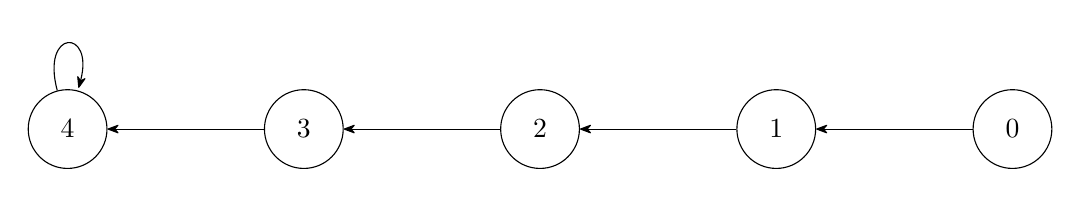
\begin{tikzpicture}[>={Stealth[round]}, node distance=2cm and 1cm, every node/.style={circle, draw, minimum size=1cm}]
    % Define vertices
    \node (v0) at (0, 0) {4};
    \node (v1) at (3, 0) {3};
    \node (v2) at (6, 0) {2};
    \node (v3) at (9, 0) {1};
    \node (v4) at (12, 0) {0};
    
    % Draw edges
    \draw [->] (v1) to (v0); % Edge 1 -> 0
    \draw [->] (v2) to (v1); % Edge 2 -> 1
    \draw [->] (v3) to (v2); % Edge 3 -> 2
    \draw [->] (v4) to (v3); % Edge 4 -> 3
    \draw[->] (v0) edge[loop above] (v0); % Self-loop at 0
\end{tikzpicture}
}
\end{center}
\ \\
\begin{center}   
$G_g: \;$
\resizebox{!}{3em}{
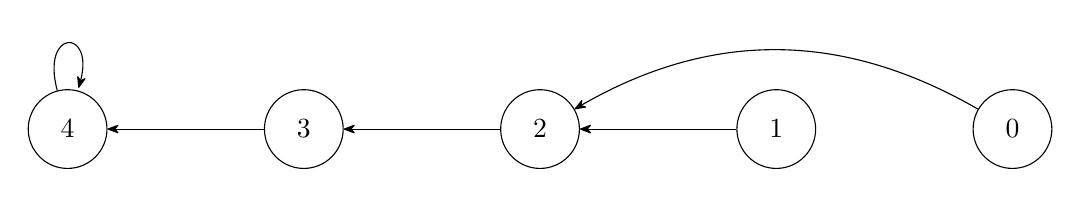
\begin{tikzpicture}[>={Stealth[round]}, node distance=2cm and 1cm, every node/.style={circle, draw, minimum size=1cm}]
    % Define vertices
    \node (v0) at (0, 0) {4};
    \node (v1) at (3, 0) {3};
    \node (v2) at (6, 0) {2};
    \node (v3) at (9, 0) {1};
    \node (v4) at (12, 0) {0};
    
    % Draw edges
    \draw [->] (v1) to (v0); % Edge 1 -> 0
    \draw [->] (v2) to (v1); % Edge 2 -> 1
    \draw [->] (v3) to (v2); % Edge 3 -> 2
    \draw [->] (v4) edge[bend right] (v2); % Edge 4 -> 2
    \draw[->] (v0) edge[loop above] (v0); % Self-loop at 0
\end{tikzpicture}
}
\end{center}
\end{example}


\bibliographystyle{alpha}
\bibliography{biblio}

\end{document}


%\home{https://emilyriehl.github.io/infinity-cosmos}
%\github{https://github.com/emilyriehl/infinity-cosmos}
%\dochome{https://emilyriehl.github.io/infinity-cosmos/docs}

\title{Composition Lemma}
\author{Edinah Gnang}
\author{Parikshit Chalise}

\begin{document}
\linenumbers
\maketitle
\tableofcontents

`% In this file you should put the actual content of the blueprint.
% It will be used both by the web and the print version.
% It should *not* include the \begin{document}
%
% If you want to split the blueprint content into several files then
% the current file can be a simple sequence of \input. Otherwise It
% can start with a \section or \chapter for instance.

\chapter{\texorpdfstring{Composition Lemma}{Composition Lemma}}

\section{Overview}
The \textit{Composition Lemma} was developed and refined over 6 years, beginning in 2018, as a novel approach to settle in the affirmative the \textit{Graceful Tree Conjecture}. The first of such papers was posted in \cite{gnang2020gracefullabelingstrees} by Gnang. A further developed series of papers resolving the same conjecture again appeared in \cite{gnang2022compositionlemma} and \cite{gnang2023proofkotzigringelrosaconjecture}. Recently, the same method has been applied to settle other longstanding conjectures in \cite{chalise2024treenedgesdecomposes} and \cite{chalise2024prooftreepackingconjecture}. We comment that the series of papers shared on the open-source platform arXiv reflect the evolving landscape of Gnang's thought process, and the frequent re-uploads were driven by the natural progression and refinement of ideas. However, we recognize that these numerous edits may have unintentionally caused confusion and raised questions regarding the success of the method. In the current work, we aim to address these concerns by presenting a detailed blueprint of the proof, with the goal of formalizing it in Lean4.

\section{Functional Directed Graphs}\label{sec:Functional Directed Graphs}
For notational convenience, let $\mathbb{Z}_{n}$ denote the set whose members are the smallest $n$ non-negative integers, i.e.,
\begin{equation}
\mathbb{Z}_{n}:=\big\{0,\ldots,\,n-1\big\}.
\end{equation}
For a function $f:\mathbb{Z}_{m}\to\mathbb{Z}_{n}$, we write $f\in\mathbb{Z}_{n}^{\mathbb{Z}_{m}}$.
For $X\subseteq\mathbb{Z}_{m}$, $f(X)$ denotes the image of $X$
under $f$, i.e.,
\begin{equation}
f(X)=\{f(i):i\in X\},
\end{equation}
and $|f(X)|$ denotes its
cardinality. For $Y\subseteq\mathbb{Z}_{n}\ensuremath{,}f^{-1}(Y)$
denotes the pre-image of $Y$ under $f$ i.e.
\begin{equation}
f^{-1}(Y)=\{j\in\mathbb{Z}_{m}:f(j)\in Y\}
\end{equation}
\begin{definition}[Functional digraphs]\label{defn:functional-directed-graphs}
% REVIEW THE LEAN LABELS BELLOW:
  %\lean{}
  %\leanok
  %\uses{defn:standard-simplex}
For an arbitrary $f\in \mathbb{Z}_n^{\mathbb{Z}_n}$, the \emph{functional directed graph} prescribed by $f$, denoted $G_f$, is such that the vertex set $V(G_f)$ and the directed edge set $E(G_f)$ are respectively as follows:
\[
V(G_f) = \mathbb{Z}_n, \; E(G_f) = \{(v,f(v)):v \in \mathbb{Z}_n\}.
\]
\end{definition}
\begin{definition}[Graceful functional digraphs]\label{defn:graceful-functional-graphs}
  %\lean{}
  %\leanok
  %\uses{defn:functional-directed-graphs}
The functional directed graph prescribed by $f\in\mathbb{Z}_{n}^{\mathbb{Z}_{n}}$ is graceful if there exist
a bijection $\sigma\in \text{S}_n \subset
 \mathbb{Z}_{n}^{\mathbb{Z}_{n}}$ such that
\begin{equation}
\big\{\left|\sigma f\sigma^{-1}(i)-i\right|:i\in\mathbb{Z}_{n}\big\}=\mathbb{Z}_{n}.
\end{equation}
If $\sigma=\text{id}$ (the identity function), then $G_{f}$ --- the functional directed graph prescribed by $f$ --- is gracefully labeled. 
\end{definition}
\begin{defn}[Automorphism group]\label{defn:aut-functional-graphs}
  %\lean{}
  %\leanok
  %\uses{defn:functional-directed-graphs}
For a functional directed graph $G_f$, its automorphism group, denoted $\text{Aut}\left(G_f\right)$, is defined as follows:
\[
\text{Aut}(G_{f})=\big\{\sigma\in\text{S}_{n}:\{\big(i,f(i)\big):i\in\mathbb{Z}_{n}\}=\{\big(j,\sigma f\sigma^{-1}(j)\big):j\in\mathbb{Z}_{n}\}\big\}.
\]
For a polynomial $P \in \mathbb{C}[x_0, \ldots, x_{n-1}]$, its automorphism group, is the stablizer of $P$ and denoted $\text{Aut($P$)}$. Formally defined as follows:
\[
\text{Aut}\left(P\right)=\large\{\sigma\in\text{S}_{n}:P\left(x_{0},\ldots,x_{i},\ldots,x_{n-1}\right)=P\left(x_{\sigma(0)},\ldots,x_{\sigma(i)},\ldots,x_{\sigma(n-1)}\right)\large\}.
\]
\end{defn}
\begin{definition}[Graceful re-labelings]\label{defn:graceful-functional-graphs-set}
  %\lean{}
  %\leanok
  %\uses{defn:functional-directed-graphs, defn:graceful-functional-graphs}
The set of distinct gracefully labeled functional directed graphs isomorphic to $G_{f}$ is 
\[
\text{GrL}\left(G_{f}\right)\,:=\left\{ G_{\sigma f\sigma^{-1}}:\begin{array}{c}
\sigma\text{ is a representative of a coset in }\nicefrac{\text{S}_{n}}{\text{Aut}\left(G_{f}\right)}\text{ and }\\
\mathbb{Z}_{n}=\left\{ \left|\sigma f\sigma^{-1}\left(i\right)-i\right|\,:\,i\in\mathbb{Z}_{n}\right\} 
\end{array}\right\} 
\]
\end{definition}
\begin{definition}[Complementary labeling involution]\label{defn:complementary-labeling-symmetry}
  %\lean{}
  %\leanok
  %\uses{defn:functional-directed-graphs, defn:graceful-functional-graphs}
If $\varphi=n-1-\text{id}$, i.e. $\varphi \in \mathbb{Z}_{n}^{\mathbb{Z}_{n}}$ such that
\[
\varphi(i)=n-1-i,\, \forall \,i\in \mathbb{Z}_{n},
\]
The complementary labeling involution is defined as the map whose domain and codomain is $\mathbb{Z}_{n}^{\mathbb{Z}_{n}}$ and is prescribed by
\[
f \mapsto \varphi f \varphi^{-1},
\]
for an arbitrary $f\in\mathbb{Z}_{n}^{\mathbb{Z}_{n}}$.
\end{definition}
Observe that for all $f\in \mathbb{Z}_{n}^{\mathbb{Z}_{n}}$ the complementary labeling involution fixes the induced edge label of each edge as seen from the equality
\begin{equation}
\left|f(i)-i\right|=\left|\varphi f(i)-\varphi(i)\right|,\quad\forall\,i\in\mathbb{Z}_{n}.
\end{equation}
In other words, induced edge labels are fixed by the vertex relabeling effected by $\varphi$. We call this induced edge label symmetry the \emph{complementary labeling symmetry} of the functional directed graph $G_f$.

\section{Quotient-Remainder Theorem and Lagrange Interpolation}\label{sec:QRT}
 \begin{proposition}[Multivariate Quotient-Remainder]\label{prop:multivariate-quotient-remainder}
  %\lean{Algebra.Polynomial.FieldDivision}
  %\leanok
  %\uses{}
Let $d(x)\in\mathbb{C}[x]$ be a degree $n$ monic polynomial with
simple roots, i.e.,
\begin{equation}
d(x)=\prod_{i\in\mathbb{Z}_{n}}(x-\alpha_{i})\;\text{ and }\:0\ne\prod_{0\le u<v<n}(\alpha_{v}-\alpha_{u}),
\end{equation}
where $\{\alpha_{u}:u\in\mathbb{Z}_{n}\}\subset\mathbb{C}$. 
For
all $P\in\mathbb{C}[x_{0},\ldots,x_{m-1}]$, there exists a unique remainder
$r(x_{0},\ldots,x_{m-1})\in\mathbb{C}[x_{0},\ldots,x_{m-1}]$ of degree
at most $n-1$ in each variable such that for quotients: $\big\{ q_{k}(x_{0},\ldots,x_{n-1}):k\in\mathbb{Z}_{n}\big\}\subset\mathbb{C}[x_{0},\ldots,x_{n-1}]$, we have
\begin{equation}
P(x_{0},\ldots,x_{m-1})= r(x_{0},\ldots,x_{m-1})+\sum_{u\in\mathbb{Z}_{m}}q_{u}(x_{0},\ldots,x_{m-1})\,d(x_{u}).
\end{equation}
 \end{proposition}
\begin{proof}
  %\leanok
We prove by induction on the number of variables that the remainder admits the expansion
\begin{equation}
r(x_{0},\ldots,x_{m-1})=\sum_{g\in\mathbb{Z}_{n}^{\mathbb{Z}_{m}}}P(\boldsymbol{\alpha}_{g})\prod_{i\in\mathbb{Z}_{m}}\left(\prod_{j_{i}\in\mathbb{Z}_{n}\backslash\{g(i)\}}\bigg(\frac{x_{i}-\alpha_{j_{i}}}{\alpha_{g(i)}-\alpha_{j_{i}}}\bigg)\right),
\end{equation}
where for notational convenience $P(\alpha_{g}):=P(\alpha_{g(0)},\ldots,\alpha_{g(m-1)})$.
The base case stems from the univariate quotient-remainder theorem over the field $\mathbb{C}$. The univariate-quotient remainder theorem over the field $\mathbb{C}$ asserts that there exist
a unique quotient-remainder pair $\big(q(x_{0}),\,r(x_{0})\big)\in\mathbb{C}[x_{0}]\times\mathbb{C}[x_{0}]$
subject to
\begin{equation}
H(x_{0})=q(x_{0})\,d(x_{0})+r(x_{0}),
\end{equation}
where $r(x_{0})\in\mathbb{C}[x_{0}]$ is of degree at most $n-1$.
It is completely determined by its evaluation over $\{\alpha_{i}:i\in\mathbb{Z}_{n}\}$,
and by Lagrange interpolation we have 
\begin{equation}
r(x_{0})=\sum_{g\in\mathbb{Z}_{n}^{\mathbb{Z}_{1}}}H(\alpha_{g(0)})\prod_{j_{0}\in\mathbb{Z}_{n}\backslash\{g(0)\}}\bigg(\frac{x_{0}-\alpha_{j_{0}}}{\alpha_{g(0)}-\alpha_{j_{0}}}\bigg),
\end{equation}
thus establishing the claim in the base case. For the induction step,
assume as our induction hypothesis that for all $F\in\mathbb{C}\left[x_{0},\ldots,x_{m-1}\right]$,
we have
\begin{equation}
F=\sum_{k\in\mathbb{Z}_{m}}q_{k}(x_{0},\ldots,x_{m-1})\,d(x_{k})+\sum_{g\in\mathbb{Z}_{n}^{\mathbb{Z}_{m}}}F(\alpha_{g})\prod_{i\in\mathbb{Z}_{m}}\left(\prod_{j_{i}\in\mathbb{Z}_{n}\backslash\left\{ g(i)\right\} }\left(\frac{x_{i}-\alpha_{j_{i}}}{\alpha_{g(i)}-\alpha_{j_{i}}}\right)\right).
\end{equation}
We proceed to show that the hypothesis implies that every polynomial in
$m+1$ variables also admits a similar expansion, thus establishing
the desired claim. Consider a polynomial $H \in \mathbb{C}[x_{0},\ldots,x_{m}]$. We view $H$ as a univariate polynomial in the variable $x_{m}$ whose coefficients lie in the field of fraction $\mathbb{C}(x_{0},\ldots,x_{m-1})$.
The univariate quotient-remainder theorem over the field of fractions $\mathbb{C}(x_{0},\ldots,x_{m-1})$ asserts that
there exit a unique quotient-remainder pair
\[
\big(q(x_{m}),\,r(x_{m})\big)\in\big(\mathbb{C}(x_{0},\ldots,x_{m-1})\big)[x_{m}]\times\big(\mathbb{C}(x_{0},\ldots,x_{m-1})\big)[x_{m}]
\]
subject to
\begin{equation}
H\big(x_{0},\ldots,x_{m}\big)=q(x_{0},\ldots,x_{m})\,d(x_{m})+r(x_{0},\ldots,x_{m}),
\end{equation}
where $r\left(x_{0},\ldots,x_{m}\right)\in\big(\mathbb{C}(x_{0},\ldots,x_{m-1})\big)[x_{m}]$
is of degree at most $n-1$ in the variable $x_{m}$. We write 
\begin{equation}
r\left(x_{0},\ldots,x_{m}\right)=\sum_{k\in\mathbb{Z}_{n}}a_{k}\left(x_{0},\ldots,x_{m-1}\right)\,(x_{m})^{k}.
\end{equation}
We now show that coefficients $\big\{ a_k(x_{0},\ldots,x_{m-1}):k\in \mathbb{Z}_n \big\}$ all lie in the polynomial ring $\mathbb{C}[x_{0},\ldots,x_{m-1}]$
via the equality 
\begin{equation}
\bigg(\text{Vander}\left(\begin{array}{c}
\alpha_{0}\\
\vdots\\
\alpha_{u}\\
\vdots\\
\alpha_{n-1}
\end{array}\right)\bigg)\cdot\left(\begin{array}{c}
a_{0}\left(x_{0},\ldots,x_{m-1}\right)\\
\vdots\\
a_{u}\left(x_{0},\ldots,x_{m-1}\right)\\
\vdots\\
a_{n-1}\left(x_{0},\ldots,x_{m-1}\right)
\end{array}\right)=\left(\begin{array}{c}
H(x_{0},\ldots,x_{m-1},\alpha_{0})\\
\vdots\\
H(x_{0},\ldots,x_{m-1},\alpha_{u})\\
\vdots\\
H(x_{0},\ldots,x_{m-1},\alpha_{n-1})
\end{array}\right),
\end{equation}
where 
\begin{equation}
\bigg(\text{Vander}\left(\begin{array}{c}
\alpha_{0}\\
\vdots\\
\alpha_{u}\\
\vdots\\
\alpha_{u}
\end{array}\right)\bigg)\left[i,j\right]=(\alpha_{i})^{j},\ \forall\,0\le i,j<n.
\end{equation}
Since the Vandermonde matrix is invertible by the fact
\begin{equation}
0\ne\det\bigg(\text{Vander}\left(\begin{array}{c}
\alpha_{0}\\
\vdots\\
\alpha_{u}\\
\vdots\\
\alpha_{u}
\end{array}\right)\bigg)=\prod_{0\le u<v<n}(\alpha_{v}-\alpha_{u}),
 \end{equation}
we indeed have 
\begin{equation}
\left(\begin{array}{c}
a_{0}\left(x_{0},\ldots,x_{m-1}\right)\\
\vdots\\
a_{u}\left(x_{0},\ldots,x_{m-1}\right)\\
\vdots\\
a_{n-1}\left(x_{0},\ldots,x_{m-1}\right)
\end{array}\right)=\bigg(\text{Vander}\left(\begin{array}{c}
\alpha_{0}\\
\vdots\\
\alpha_{u}\\
\vdots\\
\alpha_{u}
\end{array}\right)\bigg)^{-1}\cdot\left(\begin{array}{c}
H(x_{0},\ldots,x_{m-1},\alpha_{0})\\
\vdots\\
H(x_{0},\ldots,x_{m-1},\alpha_{u})\\
\vdots\\
H(x_{0},\ldots,x_{m-1},\alpha_{n-1})
\end{array}\right).
\end{equation}
Therefore, we have 
\begin{equation}
H\big(x_{0},\ldots,x_{m}\big)
= q_{m}\big(x_{0},\ldots,x_{m}\big)\,d(x_{m})+\sum_{g(m)\in\mathbb{Z}_{n}}H\big(x_{0},\ldots,x_{m-1},\alpha_{g(m)}\big)\prod_{j\in\mathbb{Z}_{n}\backslash\{g(m)\}}\left(\frac{x_{m}-\alpha_{j_{m}}}{\alpha_{g(m)}-\alpha_{j_{m}}}\right).
\end{equation}
Applying the induction hypothesis to coefficients
\[
\left\{ H\left(x_{0},\ldots,x_{m-1},\alpha_{g\left(m\right)}\right): \alpha_{g\left(m\right)}\in\mathbb{C}\right\} \subset\mathbb{C}[x_{0},\ldots,x_{m-1}]
\]
yields the desired expansion. Finally, quotients $\big\{ q_{k}(x_{0},\ldots,x_{m-1}):k\in\mathbb{Z}_{m}\big\}$ lie in the polynomial ring $\mathbb{C}[x_{0},\ldots,x_{m-1}]$ since the polynomial $H(x_0,\ldots,x_{m-1})-r(x_0,\ldots,x_{m-1})$ lies in the ideal generated by members of the set $\big\{ d(x_{u}):u\in\mathbb{Z}_{m}\big\}$.
\end{proof}
\begin{proposition}[Ring Homomorphism]\label{prop:ring-homomorphism}
  %\lean{Algebra.Polynomial.FieldDivision}
  %\leanok
  %\uses{}
For an arbitrary $H\in\mathbb{C}\left[x_{0},\ldots,x_{n-1}\right]$, let $\overline{H}$ denote
the {remainder} of the congruence class 
\[
H\text{ modulo the ideal generated by }\left\{ d(x_{i}):i\in\mathbb{Z}_{n}\right\} ,
\]
where
\[
d(x)=\prod_{i\in\mathbb{Z}_{n}}(x-\alpha_{i})\;\text{ and }\:0\ne\prod_{0\le u<v<n}(\alpha_{v}-\alpha_{u}),
\]
Then the following hold:
\begin{enumerate}
    \item For all $g\in\mathbb{Z}_{n}^{\mathbb{Z}_{n}}$, we have $\overline{H}(\boldsymbol{\alpha}_g)=H(\boldsymbol{\alpha}_g)$. 
    \item If $H = H_0 + H_1,$ where $H_0, H_1 \in \mathbb{C}\left[x_{0},\ldots,x_{n-1}\right]$, then $\overline{H_0} + \overline{H_1} = \overline{H}$.
    \item If $H = H_0 \cdot H_1,$ where $H_0, H_1 \in \mathbb{C}\left[x_{0},\ldots,x_{n-1}\right]$,  then $ \overline{H} \equiv \overline{H_0} \cdot \overline{H_1}$.
\end{enumerate}
 \end{proposition}
\begin{proof}
  %\leanok
  The first claim follows from Proposition \ref{prop:multivariate-quotient-remainder} for we see that the divisor vanishes over the lattice. To prove the second claim we recall that
  \[
\overline{H}=\sum_{g\in\mathbb{Z}_{n}^{\mathbb{Z}_{n}}}H(\boldsymbol{\alpha}_{g})\prod_{i\in\mathbb{Z}_{n}}\left(\prod_{j_{i}\in\mathbb{Z}_{n}\backslash\{g(i)\}}\bigg(\frac{x_{i}-\alpha_{j_{i}}}{\alpha_{g(i)}-\alpha_{j_{i}}}\bigg)\right),
  \]
  \[
  \implies\overline{H}=\sum_{g\in\mathbb{Z}_{n}^{\mathbb{Z}_{n}}}\big(H_{0}(\boldsymbol{\alpha}_{g})+H_{1}(\boldsymbol{\alpha}_{g})\big)\prod_{i\in\mathbb{Z}_{n}}\left(\prod_{j_{i}\in\mathbb{Z}_{n}\backslash\{g(i)\}}\bigg(\frac{x_{i}-\alpha_{j_{i}}}{\alpha_{g(i)}-\alpha_{j_{i}}}\bigg)\right),
  \]
  \[
  \implies\overline{H}=\sum_{k\in\mathbb{Z}_{2}}\sum_{g\in\mathbb{Z}_{n}^{\mathbb{Z}_{n}}}H_{k}(\boldsymbol{\alpha}_{g})\prod_{i\in\mathbb{Z}_{n}}\left(\prod_{j_{i}\in\mathbb{Z}_{n}\backslash\{g(i)\}}\bigg(\frac{x_{i}-\alpha_{j_{i}}}{\alpha_{g(i)}-\alpha_{j_{i}}}\bigg)\right).
  \]
  Thus $\overline{H_0} + \overline{H_1} = \overline{H}$ as claimed. Finally the fact (iii) is a straightforward consequence of Proposition \ref{prop:Orthogonality}, which is proved next.
\end{proof}
\begin{proposition}
 \label{prop:Orthogonality}
  %\lean{}
  %\leanok
  %\uses{prop:multivariate-quotient-remainder}   
 Let $f,g \in\mathbb{Z}_{n}^{\mathbb{Z}_{n}}$. For congruence classes prescribed modulo the ideal generated by $\{d(x_{i}):i \in \Z_n\}$, if
\[
d(x)=\prod_{i\in\mathbb{Z}_{n}}(x-\alpha_{i})\;\text{ such that }\:0\ne\prod_{0\le u<v<n}(\alpha_{v}-\alpha_{u}),
\]
then
\[
L_{f}({\bf x})\cdot L_{g}({\bf x})\equiv\begin{cases}
L_{f}({\bf x}) & \text{if }f=g\\
0 & \text{otherwise,}
\end{cases}
\]
\end{proposition}
\begin{proof} Observe that
\[
L_{f}(\mathbf{x})\cdot L_{g}(\mathbf{x})\;=\;\prod_{i\in\mathbb{Z}_{n}}\bigg(\big(c_{i,f}\frac{d(x_{i})}{x_{i}-\alpha_{f(i)}}\big)\big(c_{i,g}\frac{d(x_{i})}{x_{i}-\alpha_{g(i)}}\big)\bigg),
\]
where
\[
c_{i,f}=\prod_{j_{i}\in\mathbb{Z}_{n}\backslash\{f(i)\}}\big(\alpha_{f(i)}-\alpha_{j_{i}}\big)^{-1}\quad\text{ and }\quad c_{i,g}=\prod_{j_{i}\in\mathbb{Z}_{n}\backslash\{g(i)\}}\big(\alpha_{g(i)}-\alpha_{j_{i}}\big)^{-1}.
\]
If $f \neq g$, then there exists $j \in \Z_n$ such that $f(j)\neq g(j)$ and $L_{f}(\mathbf{x})\cdot L_{g}(\mathbf{x})$ is a multiple of $d(x_{j})$,
as a result of which we obtain $L_{f}(\mathbf{x})\cdot L_{g}(\mathbf{x}) \equiv 0$. Alternatively if $f = g$, then
\[
L_{f}(\mathbf{x})\cdot L_{g}(\mathbf{x})=\big(L_{f}(\mathbf{x})\big)^{2}=L_{f}(\mathbf{x})+\bigg(\big(L_{f}(\mathbf{x})\big)^{2}-L_{f}(\mathbf{x})\bigg).
\]
We now show that $\big(L_{f}(\mathbf{x})\big)^{2}-L_{f}(\mathbf{x})\equiv 0$ modulo the ideal generated by $\left\{ d(x_{i}):i\in\mathbb{Z}_{n}\right\}$.
\begin{align*}
\big(L_{f}(\mathbf{x})\big)^{2}-L_{f}(\mathbf{x})\; & =\;L_{f}(\mathbf{x})\left(L_{f}(\mathbf{x})-1\right)\\
 & =\;L_{f}(\mathbf{x})\bigg(L_{f}(\mathbf{x})-\sum_{g\in\mathbb{Z}_{n}^{\mathbb{Z}_{n}}}L_{g}\left({\bf x}\right)\bigg)\\
 & =\;-L_{f}(\mathbf{x})\bigg(\sum_{g\in\mathbb{Z}_{n}^{\mathbb{Z}_{n}}\setminus\{f\}}L_{g}\left({\bf x}\right)\bigg)\\
 & \equiv\;0,
\end{align*}
where the latter congruence identity stems from the prior setting where $f\ne g$.
\end{proof}

\begin{defn}[Polynomial of Grace]\label{defn:polynomial-grace-definition} We define $P_f \in \mathbb{C}[x_0, \ldots, x_{n-1}]$ for all $f \in \mathbb{Z}_n^{\mathbb{Z}_n}$ as follows:
\begin{equation}
    P_f(\mathbf{x}) \coloneq \underbrace{\prod_{0\le u<v<n}(x_{v}-x_{u})}_{V(x_0,\ldots,x_{n-1})}\,\underbrace{\prod_{0\le u<v<n}\big((x_{f(v)}-x_{v})^{2}-(x_{f(u)}-x_{u})^{2}\big)}_{E_f(x_0,\ldots,x_{n-1})}.
\end{equation}
\end{defn}
\begin{defn}[Congruence class]\label{defn:polynomial-congruence}
  %\lean{}  %\leanok
  %\uses{prop:multivariate-quotient-remainder}
For polynomials $P,Q \in \mathbb{C}[x_0, \ldots, x_{n-1}]$, if
\begin{equation}
P({\bf x}) \equiv \; Q({\bf x}) \; \mod\bigg\{\prod_{j\in\mathbb{Z}_{n}}(x_{i}-j):i\in\mathbb{Z}_{n}\bigg\},
\end{equation}
we simply write $P \equiv Q$.
\end{defn}
 Unless otherwise stated, all subsequent congruence identities are prescribed modulo the ideal of polynomials generated by members of the set
\[
\bigg\{\prod_{j\in\mathbb{Z}_{n}}(x_{i}-j):i\in\mathbb{Z}_{n}\bigg\}
\]
\begin{proposition}[Certificate of Grace]\label{prop:polynomial-grace-certificate}
  %\lean{}
  %\leanok
  %\uses{defn:polynomial-grace-definition, defn:polynomial-congruence, prop:multivariate-quotient-remainder}
Let $f\in\mathbb{Z}_{n}^{\mathbb{Z}_{n}}$. The functional
directed graph $G_f$ prescribed by $f$ is graceful if and only if $P_f(\mathbf{x}) \; \not\equiv \; 0$.
\end{proposition}
\begin{proof}
Observe that the vertex Vandermonde factor $V(\mathbf{x})$ is of degree exactly $n-1$ in each variable and therefore equal
to its remainder, i.e.,
\begin{equation}\label{eq:Vf}
V(\mathbf{x})=\sum_{\theta\in\text{S}_{n}}\text{sgn}(\theta)\prod_{i\in\mathbb{Z}_{n}}(x_{i})^{\theta(i)}=\prod_{v\in\mathbb{Z}_{n}}(v!)\;\sum_{\theta\in\text{S}_{n}}\text{sgn}(\theta)\prod_{\begin{array}{c}
\substack{i\in\mathbb{Z}_{n}\\
j_{i}\in\mathbb{Z}_{n}\backslash\{\theta(i)\}
}
\end{array}}\left(\frac{x_{i}-j_{i}}{\theta(i)-j_{i}}\right),
\end{equation}
where 
\begin{equation}
\text{sgn}(\theta):=\prod_{0\le u<v<n}\left(\frac{\theta(v)-\theta(u)}{v-u}\right),\quad\forall\,\theta\in\text{S}_{n}.
\end{equation}
When $n>2$, for every $f\in\mathbb{Z}_{n}^{\mathbb{Z}_{n}}$, the induced edge label Vandermonde factor $E_f(\mathbf{x})$
is of degree $>(n-1)$ in some of its variables. Therefore, by Proposition  \ref{prop:multivariate-quotient-remainder}, we have
\begin{equation}\label{eq:Ef}
E_{f}(\mathbf{x})=\sum_{l\in\mathbb{Z}_{m}}q_{l}(\mathbf{x})\prod_{k\in\mathbb{Z}_{n}}(x_{l}-k)+\prod_{v\in\mathbb{Z}_{n}}(v!)\frac{(n-1+v)!}{(2v)!}\sum_{\begin{array}{c}
g\in\mathbb{Z}_{n}^{\mathbb{Z}_{n}}\\
|gf-g|\in\text{S}_{n}
\end{array}}\text{sgn}(|gf-g|)\prod_{\begin{array}{c}
\substack{i\in\mathbb{Z}_{n}\\
j_{i}\in\mathbb{Z}_{n}\backslash\{g(i)\}
}
\end{array}}\big(\frac{x_{i}-j_{i}}{g(i)-j_{i}}\big).
\end{equation}
Observe that by the expansions in \ref{eq:Vf} and \ref{eq:Ef}, 
\[
P_{f}(\mathbf{x})=\sum_{l\in\mathbb{Z}_{m}}q_{l}(\mathbf{x})V(\mathbf{x})\prod_{k\in\mathbb{Z}_{n}}(x_{l}-k)+
\]
\[
\bigg(\prod_{v\in\mathbb{Z}_{n}}v!\sum_{\theta\in\text{S}_{n}}\text{sgn}(\theta)\prod_{\begin{array}{c}
\substack{i\in\mathbb{Z}_{n}\\
j_{i}\in\mathbb{Z}_{n}\backslash\{\theta(i)\}
}
\end{array}}\big(\frac{x_{i}-j_{i}}{\theta(i)-j_{i}}\big)\bigg)\bigg(\prod_{v\in\mathbb{Z}_{n}}(v!)\frac{(n-1+v)!}{(2v)!}\sum_{\begin{array}{c}
g\in\mathbb{Z}_{n}^{\mathbb{Z}_{n}}\\
|gf-g|\in\text{S}_{n}
\end{array}}\text{sgn}(|gf-g|)\prod_{\begin{array}{c}
\substack{i\in\mathbb{Z}_{n}\\
j_{i}\in\mathbb{Z}_{n}\backslash\{g(i)\}
}
\end{array}}\big(\frac{x_{i}-j_{i}}{g(i)-j_{i}}\big)\bigg).
\]
is congruent to
\begin{equation} \label{eq:graceful-evaluation}
\prod_{v\in\mathbb{Z}_{n}}(v!)^{2}\frac{(n-1+v)!}{(2v)!}\sum_{\begin{array}{c}
\substack{\sigma\in\text{S}_{n}\\
\text{s.t.}\\
\left|\sigma f-\sigma\right|\in\text{S}_{n}
}
\end{array}}\text{sgn}(\sigma\left|\sigma f-\sigma\right|)\prod_{\begin{array}{c}
\substack{i\in\mathbb{Z}_{n}\\
j_{i}\in\mathbb{Z}_{n}\backslash\{\sigma(i)\}
}
\end{array}}\big(\frac{x_{i}-j_{i}}{\sigma(i)-j_{i}}\big),
\end{equation}
where the permutation $|\sigma f-\sigma |$ denotes the induced edge label permutation associated with a graceful relabeling $G_{\sigma f\sigma^{-1}}$ of $G_f$.
The congruence above stems from Prop. \ref{prop:Orthogonality}. A graceful labeling necessitates the integer coefficient
\[
\prod_{0\le i<j<n}(j-i)\big(j^{2}-i^{2})=\prod_{0\le i<j<n}(j-i)^{2}(j+i)=\prod_{v\in\mathbb{Z}_{n}}\left(v!\right)^{2}\frac{\left(n-1+v\right)!}{\left(2v\right)!} \neq 0,
\]
thus establishing the desired claim.
\end{proof}
\begin{example} We present an example of a path on 5 vertices. This is known to be graceful, so we expect a non-zero remainder.
\ \\
\begin{center}   
\resizebox{!}{3em}{
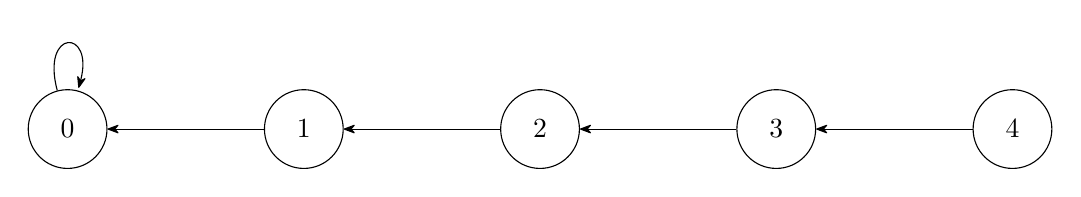
\begin{tikzpicture}[>={Stealth[round]}, node distance=2cm and 1cm, every node/.style={circle, draw, minimum size=1cm}]
    % Define vertices
    \node (v0) at (0, 0) {0};
    \node (v1) at (3, 0) {1};
    \node (v2) at (6, 0) {2};
    \node (v3) at (9, 0) {3};
    \node (v4) at (12, 0) {4};
    
    % Draw edges
    \draw [->] (v1) to (v0); % Edge 1 -> 0
    \draw [->] (v2) to (v1); % Edge 2 -> 1
    \draw [->] (v3) to (v2); % Edge 3 -> 2
    \draw [->] (v4) to (v3); % Edge 4 -> 3
    \draw[->] (v0) edge[loop above] (v0); % Self-loop at 0
\end{tikzpicture}
}
\end{center}
Run the SageMath script \texttt{ex1325.sage} to verify.
\end{example}

\section{The Composition Lemma}

\begin{prop}[Composition Inequality]\label{prop:composition-lemma-ineq}
  %\lean{}
  %\leanok
  %\uses{defn:graceful-functional-graphs, defn:graceful-functional-graphs-set, prop:multivariate-quotient-remainder, defn:polynomial-grace-definition, defn:polynomial-congruence, prop:polynomial-grace-certificate}
Consider an arbitrary $f\in\mathbb{Z}_{n}^{\mathbb{Z}_{n}}$ subject to the fixed point condition
$\left|f^{\left(n-1\right)}\left(\mathbb{Z}_{n}\right)\right|=1$. The following statements are equivalent:
\begin{enumerate}
    \item 
    \[
    \max_{\sigma\in\text{S}_{n}}\big|\{|\sigma f^{(2)}\sigma^{-1}(i)-i|:i\in\mathbb{Z}_{n}\}\big|\le\max_{\sigma\in\text{S}_{n}}\big|\{|\sigma f\sigma^{-1}(i)-i|:i\in\mathbb{Z}_{n}\}\big|.
    \]
    \item
    \[
    P_{f^{(2)}} ({\bf x}) \not\equiv 0  \implies  P_{f} ({\bf x}) \not\equiv 0.
    \]
    \item 
    \[
    \text{GrL}(G_f) \neq \varnothing
    \]
\end{enumerate}    
\end{prop}
\begin{proof}
If $f\in\mathbb{Z}_{n}^{\mathbb{Z}_{n}}$ is identically constant,
then $G_{f}$ is graceful. We see this from the fact that the functional
digraph of the identically zero function is gracefully labeled and the fact that
functional digraphs of identically constant functions are all isomorphic. It follows
that all functional directed graphs having diameter less than $3$ are graceful. Consequently,
all claims hold for all functional digraphs of diameter less than $3$. We now turn our attention
to functional trees of diameter greater or equal to $3$. 
It follows by definition 
\begin{equation}
n=\max_{\sigma\in\text{S}_{n}}\big|\{|\sigma f\sigma^{-1}(i)-i|:i\in\mathbb{Z}_{n}\}\big|\iff P_{f}({\bf x})\not\equiv0\iff\text{GrL}(G_{f})\neq\varnothing.
\end{equation}
We now proceed to show (i) $\iff$ (iii). The backward claim is the simplest of the two claims. We see
that if $f$ is contractive, so too is $f^{(2)}$. Then 
assertions
\begin{equation}
n=\max_{\sigma\in\text{S}_{n}}\big|\{|\sigma f^{(2)}\sigma^{-1}(i)-i|:i\in\mathbb{Z}_{n}\}\big|\text{  and  }n=\max_{\sigma\in\text{S}_{n}}\big|\{|\sigma f\sigma^{-1}(i)-i|:i\in\mathbb{Z}_{n}\}\big|
\end{equation}
indeed implies the inequality
\begin{equation}
\max_{\sigma\in\text{S}_{n}}\big|\{|\sigma f^{(2)}\sigma^{-1}(i)-i|:i\in\mathbb{Z}_{n}\}\big|\le\max_{\sigma\in\text{S}_{n}}\big|\{|\sigma f\sigma^{-1}(i)-i|:i\in\mathbb{Z}_{n}\}\big|.
\end{equation}
We now establish the forward claim by contradiction. Assume for the
sake of establishing a contradiction that for some contractive map
$f\in\mathbb{Z}_{n}^{\mathbb{Z}_{n}}$ we have 
\begin{equation}
n>\max_{\sigma\in\text{S}_{n}}\left|\left\{ |\sigma f^{(2)}\sigma^{-1}(i)-i|:i\in\mathbb{Z}_{n}\right\} \right|,
\end{equation}
for we know by the number of edges being equal to $n$ that it is impossible
 that 
\begin{equation}
n<\max_{\sigma\in\text{S}_{n}}\left|\left\{ |\sigma f^{(2)}\sigma^{-1}(i)-i|:i\in\mathbb{Z}_{n}\right\} \right|.
\end{equation}
Note that the range of $f$ is a proper subset of $\mathbb{Z}_{n}$.
By the premise that $f$ is contractive, it follows that $f^{(\left\lceil 2^{\text{lg}(n-1)}\right\rceil )}$
is identically constant and thus 
\begin{equation}
n=\max_{\sigma\in\text{S}_{n}}\left|\left\{ |\sigma f^{(\left\lceil 2^{\text{lg}(n-1)}\right\rceil )}\sigma^{-1}(i)-i|:i\in\mathbb{Z}_{n}\right\} \right|,
\end{equation}
where lg denotes the logarithm base $2$. Consequently there must
be some integer $0\le\kappa<\text{lg}(n-1)$ such that 
\begin{equation}
\max_{\sigma\in\text{S}_{n}}\left|\left\{ |\sigma f^{(\left\lceil 2^{\kappa}\right\rceil )}\sigma^{-1}(i)-i|:i\in\mathbb{Z}_{n}\right\} \right|>\max_{\sigma\in\text{S}_{n}}\left|\left\{ |\sigma f^{(\left\lceil 2^{\kappa-1}\right\rceil )}\sigma^{-1}(i)-i|:i\in\mathbb{Z}_{n}\right\} \right|.
\end{equation}
This contradicts the assertion of statement (i), thereby
establishing the backward claim. 
The exact same reasoning as above establishes (ii) $\iff$ (iii), for we have
\begin{equation}
        P_{f^{\left(\left\lceil 2^{\text{lg}(n-1)}\right\rceil \right)}} ({\bf x}) \not\equiv 0. 
\end{equation}
\end{proof}

Having assembled together the pieces required to prove our main result, we proceed to fit the pieces together to state and prove the \textit{Composition Lemma}.
\begin{lemma}[Composition Lemma]\label{lem:composition-lemma}
    %\lean{}
  %\leanok
  %\uses{defn:graceful-functional-graphs, defn:graceful-functional-graphs-set, prop:multivariate-quotient-remainder, defn:polynomial-grace-definition, defn:polynomial-congruence, prop:polynomial-grace-certificate, prop:composition-lemma-ineq}
 For all contractive  $f\in\mathbb{Z}_{n}^{\mathbb{Z}_{n}}$, i.e., functions subject to the fixed point condition
$\left|f^{\left(n-1\right)}\left(\mathbb{Z}_{n}\right)\right|=1$,
we have
\begin{equation}\label{eq:composition-lemma}
\max_{\sigma\in\text{S}_{n}}\big|\{|\sigma f^{(2)}\sigma^{-1}(i)-i|:i\in\mathbb{Z}_{n}\}\big|\le\max_{\sigma\in\text{S}_{n}}\big|\{|\sigma f\sigma^{-1}(i)-i|:i\in\mathbb{Z}_{n}\}\big|.
\end{equation}
\end{lemma}
\begin{proof}
Owing to Proposition \ref{prop:composition-lemma-ineq}, we prove the statement by establishing 
\[
    P_{f^{(2)}} ({\bf x}) \not\equiv 0  \implies  P_{f} ({\bf x}) \not\equiv 0.
\]
For simplicity, we prove a generalization of the desired claim. Assume without loss of generality that
\[
f(i)>i,\ \forall\:i\in\mathbb{Z}_{n-1}\text{  and  }f(n-1)=n-1.
\]
Further assume without loss of generality that the vertex labeled $0$ is at furthest edge distance from the root in $G_f$ (i.e. the vertex labeled $n-1$). Given that the diameter of $G_{f}$ is greater than $2$, we may also assume without loss of generality that  $f^{-1}\left(\{0\}\right)=\varnothing$
and $f^{(2)}(0)\ne f(0)$. Let the contractive
map $g\in\mathbb{Z}_{n}^{\mathbb{Z}_{n}}$ be devised from $f$ such that 
\begin{equation}
g(i)=\begin{cases}
\begin{array}{cc}
f^{(2)}(i) & \text{ if }i\in f^{-1}\big(\{f(0)\}\big)\\
f(i) & \text{otherwise}
\end{array},\ \forall\,i\in\mathbb{Z}_{n}.\end{cases}
\end{equation}
We show that
\begin{equation} \label{eq:composition-lemma-generalized}
P_{g} ({\bf x}) \not\equiv 0  \implies  P_{f} ({\bf x}) \not\equiv 0.
\end{equation}
Note that the assertion immediately above generalizes the composition
lemma since, $f$ is only partially
iterated. More precisely, we iterate $f$ on the subset $f^{-1}\big(\{f(0)\}\big)$.
In turn, iterating (at most $n-1$ times) this generalization  of the composition lemma yields
that all functional trees are graceful, which in turn implies that the \textit{Composition Lemma} as stated in Lemma \ref{eq:composition-lemma}  holds. For notational convenience, assume without loss of generality that 
\begin{equation}
f^{-1}\big(\{f(0)\}\big)=\mathbb{Z}_{\left|f^{-1}\big(\{f(0)\}\big)\right|}\text{  and  }f(0)=\left|f^{-1}\big(\{f(0)\}\big)\right|.
\end{equation}
If the conditions stated above are not met, we relabel the vertices of $G_f$ to ensure that such is indeed the case. In the remainder of the proof let $p$ be the smallest prime subject to $2n-1\le p$. We consider the slight variant of the polynomial certificate construction given by
\[
\mathcal{P}_{f}(\mathbf{x})\coloneq\underbrace{\prod_{0\le u<v<n}(x_{v}-x_{u})}_{V(x_{0},\ldots,x_{n-1})}\,\underbrace{\prod_{i\in\mathbb{Z}_{n}}\big(\prod_{j\in\mathbb{Z}_{p}\backslash\mathbb{Z}_{n}}(x_{i}-j)\big)}_{\mathcal{S}(x_{0},\ldots,x_{n-1})}\,\underbrace{\prod_{0\le u<v<n}\bigg(\prod_{t\in\mathbb{Z}_{2}}\big((x_{f(v)}-x_{v})+(-1)^{t}(x_{f(u)}-x_{u})\big)\bigg)}_{E_{f}(x_{0},\ldots,x_{n-1})}.
\]
In which case the canonical representative of the congruence class of $\mathcal{P}_f$ modulo the polynomials ideal generated by members of the set
\[
\bigg\{\prod_{j\in\mathbb{Z}_{p}}(x_{i}-j):i\in\mathbb{Z}_{n}\bigg\}
\]
is given by
\begin{equation} \label{eq:new-graceful-evaluation}
\overline{\mathcal{P}_{f}}(\mathbf{x})=\prod_{v\in\mathbb{Z}_{n}}(v!)^{2}\frac{(n-1+v)!}{(2v)!}\prod_{i\in\mathbb{Z}_{n}}\big(\prod_{j\in\mathbb{Z}_{p}\backslash\mathbb{Z}_{n}}(i-j)\big)\sum_{\begin{array}{c}
\substack{\sigma\in\text{S}_{n}\\
\text{s.t.}\\
\left|\sigma f-\sigma\right|\in\text{S}_{n}
}
\end{array}}\text{sgn}(\sigma\left|\sigma f-\sigma\right|)\prod_{\begin{array}{c}
\substack{i\in\mathbb{Z}_{n}\\
j_{i}\in\mathbb{Z}_{p}\backslash\{\sigma(i)\}
}
\end{array}}\big(\frac{x_{i}-j_{i}}{\sigma(i)-j_{i}}\big),
\end{equation}
which is a polynomial of degree at most $p-1$ in each variable and
\[
\prod_{v\in\mathbb{Z}_{n}}(v!)^{2}\frac{(n-1+v)!}{(2v)!}\prod_{i\in\mathbb{Z}_{n}}\big(\prod_{j\in\mathbb{Z}_{p}\backslash\mathbb{Z}_{n}}(i-j)\big)\not\equiv0\mod p.
\]
A similar expansion holds for $g$, with the same coefficient up to sign. Next, roughly speaking, we show that there exist a in invertible linear transformation which  maps $\mathcal{P}_f$ to $\mathcal{P}_g$ and vice versa. For an arbitrary $h\in \mathbb{Z}_{n}^{\mathbb{Z}_{n}}$ let $A_{h}\in\{0,1\}^{n\times n}$ denote the adjacency matrix of the functional directed graph $G_h$ i.e.
\[
A_{h}[u,v]=\begin{cases}
\begin{array}{cc}
1 & \text{ if }v=h(u)\\
0 & \text{otherwise}
\end{array}, & \forall\,(u,v)\in\mathbb{Z}_{n}\times\mathbb{Z}_{n}\end{cases}.
\]
Observe that signed incidence matrices $(A_{\text{id}}-A_{f})$ and $(A_{\text{id}}-A_{g})$ of $G_f$ and $G_g$ respectively are both in Row-Echelon form. Induced edge label binomials $x_i-x_{f(i)}$ and $x_i-x_{g(i)}$ correspond to the $i$-th entry of $(A_{\text{id}}-A_{f})\cdot \mathbf{x}$ and $(A_{\text{id}}-A_{g})\cdot \mathbf{x}$ respectively. Given that $G_f$ is a functional tree, for each one of the ${n \choose 2}$ vertex pair $(i,\,j)$ where $0\le i < j <n$, there exist a unique $\mathbf{v}_{i,j}\in\{-1,0,1\}^{n\times1}$ such that
\[
(x_{j}-x_{i})=\mathbf{v}_{i,j}^{\top}\cdot (A_{\text{id}}-A_{f})\cdot\mathbf{x}.
\]
By introducing a distinct variable $y_{i,j}$ for each one of the ${n \choose 2}$ vertex pair $(i,\,j)$ where $0\le i < j <n$, we subsequently make use of the equality
\[
y_{i,j}\,(x_{j}-x_{i})=(y_{i,j}\mathbf{v}_{i,j})^{\top}\cdot(A_{\text{id}}-A_{f})\cdot\mathbf{x}.
\]
in expressing the multiple of the vertex Vandermonde factor
\[
\prod_{0\le i<j<n}y_{i,j}\,(x_{j}-x_{i})=\prod_{0\le i<j<n}\big((y_{i,j}\mathbf{v}_{i,j})^{\top}\cdot(A_{\text{id}}-A_{f})\cdot\mathbf{x}\big).
\]
Similarly the absolute induced edge label Vandermonde factor is expressed by
\[
\prod_{0\le u<v<n}\bigg(\prod_{t\in\mathbb{Z}_{2}}\big((x_{f(v)}-x_{v})+(-1)^{t}(x_{f(u)}-x_{u})\big)\bigg)=\prod_{0\le i<j<n}\,\prod_{t\in\mathbb{Z}_{2}}\bigg(\big(A_{\text{id}}[j,:]\cdot(A_{\text{id}}-A_{f})+(-1)^{t}A_{\text{id}}[i,:]\cdot(A_{\text{id}}-A_{f})\big)\cdot\mathbf{x}\bigg).
\]
Let
\[
\mathcal{P}_{f}(\mathbf{x},Y)\coloneq
\]
\[
\prod_{0\le i<j<n}\big((y_{i,j}\mathbf{v}_{i,j})^{\top}\cdot(A_{\text{id}}-A_{f})\cdot\mathbf{x}\big)\,\mathcal{S}(x_{0},\ldots,x_{n-1})\,\prod_{0\le i<j<n}\,\prod_{t\in\mathbb{Z}_{2}}\bigg(\big(A_{\text{id}}[j,:]\cdot(A_{\text{id}}-A_{f})+(-1)^{t}A_{\text{id}}[i,:]\cdot(A_{\text{id}}-A_{f})\big)\cdot\mathbf{x}\bigg).
\]

We bypass ring homomorphisms from $\mathbb{Q}[x_0,\ldots , x_{n-1}]$ to the quotient ring $\nicefrac{\mathbb{Q}[x_{0},\ldots,x_{n-1}]}{\text{Ideal generated by }\big\{\underset{j\in\mathbb{Z}_{p}}{\prod}(x_{i}-j):i\in\mathbb{Z}_{n}\big\}}$ in our analysis by switching the ground field from $\mathbb{Q}$ to the Galois field of order $p$. More precisely we work over the ring $(\nicefrac{\mathbb{Z}}{p\mathbb{Z}})[x_{0},\ldots,x_{n-1}]$ instead of $\mathbb{Q}[x_{0},\ldots,x_{n-1}]$. Over the said ring the polynomial $\mathcal{P}_f(\mathbf{x})$ is indistinguishable from $\overline{\mathcal{P}_{f}}(\mathbf{x})$ in \ref{eq:new-graceful-evaluation}.
In order for variables to be consistently treated by our proposed linear transformation, we re-express the polynomial $\mathcal{P}_{f}(\mathbf{x},Y)$ by replacing the factor $\mathcal{S}(x_{0},\ldots,x_{n-1})$
with an expression featuring instead
\[
\mathcal{S}_{r}(x_{0},\ldots,x_{r-1},x_{r},x_{r+1},\ldots,x_{n-1},Y)\coloneq\prod_{i<r}\bigg(\prod_{j\in\mathbb{Z}_{p}\backslash\mathbb{Z}_{n}}\big(-y_{i,r}\,(x_{r}-x_{i})-j\,y_{i,r}\big)\bigg)\prod_{i>r}\bigg(\prod_{j\in\mathbb{Z}_{p}\backslash\mathbb{Z}_{n}}\big(y_{r,i}\,(x_{i}-x_{r})-j\,y_{r,i}\big)\bigg),
\]
for all $r\in \mathbb{Z}_n$. In other words
\[
\mathcal{S}_{r}(x_{0},\ldots,x_{r-1},x_{r},x_{r+1},\ldots,x_{n-1},Y)=
\]
\[
\prod_{i<r}\bigg(\prod_{j\in\mathbb{Z}_{p}\backslash\mathbb{Z}_{n}}\big(-(y_{i,r}\mathbf{v}_{i,r})^{\top}\cdot(A_{\text{id}}-A_{f})\cdot\left(\begin{array}{c}
x_{0}\\
\vdots\\
x_{r-1}\\
x_{r}\\
x_{r+1}\\
\vdots\\
x_{n-1}
\end{array}\right)-j\,y_{i,r}\big)\bigg)\prod_{i>r}\bigg(\prod_{j\in\mathbb{Z}_{p}\backslash\mathbb{Z}_{n}}\big((y_{r,i}\mathbf{v}_{r,i})^{\top}\cdot(A_{\text{id}}-A_{f})\cdot\left(\begin{array}{c}
x_{0}\\
\vdots\\
x_{r-1}\\
x_{r}\\
x_{r+1}\\
\vdots\\
x_{n-1}
\end{array}\right)-j\,y_{r,i}\big)\bigg)
\]
Over the chosen ring the following equality holds
\[
\mathcal{P}_{f}(\mathbf{x},Y)=\sum_{r\in\mathbb{Z}_{n}}\mathcal{P}_{f}(\left(\begin{array}{c}
x_{0}\\
\vdots\\
x_{r-1}\\
0\\
x_{r+1}\\
\vdots\\
x_{n-1}
\end{array}\right),Y)
\]

\[
\implies \mathcal{P}_{f}(\mathbf{x},Y)=\sum_{r\in\mathbb{Z}_{n}}\prod_{0\le i<j<n}\big((y_{i,j}\mathbf{v}_{i,j})^{\top}\cdot(A_{\text{id}}-A_{f})\cdot\left(\begin{array}{c}
x_{0}\\
\vdots\\
x_{r-1}\\
0\\
x_{r+1}\\
\vdots\\
x_{n-1}
\end{array}\right)\big)\,\mathcal{S}_{r}(x_{0},\ldots,x_{r-1},0,x_{r+1},\ldots,x_{n-1},Y)\,\times
\]
\[
\prod_{0\le i<j<n}\,\prod_{t\in\mathbb{Z}_{2}}\bigg(\big(A_{\text{id}}[j,:]\cdot(A_{\text{id}}-A_{f})+(-1)^{t}A_{\text{id}}[i,:]\cdot(A_{\text{id}}-A_{f})\big)\cdot\left(\begin{array}{c}
x_{0}\\
\vdots\\
x_{r-1}\\
0\\
x_{r+1}\\
\vdots\\
x_{n-1}
\end{array}\right)\bigg).
\]
Thus we have expressed $\mathcal{P}_{f}(\mathbf{x},Y)$ as a polynomial in the entries of $Y$ as well as the ${n \choose 2}$ binomials $x_j-x_i$ where $0\le i<j<n$. Albeit the factor $\mathcal{S}_r$ features binomials $x_r-x_i$ when $i<r$ as well as binomials $x_i-x_r$ when $r<i$ where the variable $x_r$ is evaluated to zero. 

Observe that the set of row linear combinations
\[
\text{Row}_{f(0)}+\text{Row}_{i}\longrightarrow\text{Row}_{i},\ \forall\:i\in f^{-1}\big(\{f(0)\}\big).
\]
converts the incidence matrix $A_{\text{id}}-A_{f}$ to the incidence matrix $A_{\text{id}}-A_{g}$.
These row operations are in turn expressed in terms of left elementary matrix action as follows
\[
\bigg(\prod_{i\in f^{-1}\big(\{f(0)\}\big)}(A_{\text{id}}+A_{\text{id}}[:,i]\cdot A_{\text{id}}[f(0),:])\bigg)\cdot(A_{\text{id}}-A_{f})=(A_{\text{id}}-A_{g}).
\]
Consider the invertible linear transformation which effects simultaneous maps
\[
\mathbf{x}\mapsto\bigg(\prod_{i\in f^{-1}\big(\{f(0)\}\big)}(A_{\text{id}}+A_{\text{id}}[:,i]\cdot A_{\text{id}}[f(0),:])\bigg)\cdot\mathbf{x}\text{ and }y_{i,j}\mathbf{v}_{i,j}^{\top}\mapsto y_{i,j}\mathbf{v}_{i,j}^{\top}\cdot\bigg(\prod_{i\in f^{-1}\big(\{f(0)\}\big)}(A_{\text{id}}-A_{\text{id}}[:,i]\cdot A_{\text{id}}[f(0),:])\bigg).
\]
In other words the vector
\[
\left(\begin{array}{c}
\mathbf{x}\\
y_{0,1}\mathbf{v}_{0,1}\\
\vdots\\
y_{i,j}\mathbf{v}_{i,j}\\
\vdots\\
y_{n-2,n-1}\mathbf{v}_{n-2,n-1}
\end{array}\right)
\]
is mapped to
\[
\left(\big(\prod_{i\in f^{-1}\big(\{f(0)\}\big)}(A_{\text{id}}+A_{\text{id}}[:,i]\cdot A_{\text{id}}[f(0),:])\big)\oplus\bigg(I_{{n \choose 2}}\otimes\big(\prod_{i\in f^{-1}\big(\{f(0)\}\big)}(A_{\text{id}}-A_{\text{id}}[:,i]\cdot A_{\text{id}}[f(0),:])\big)^{\top}\bigg)\right)\cdot\left(\begin{array}{c}
\mathbf{x}\\
y_{0,1}\mathbf{v}_{0,1}\\
\vdots\\
y_{i,j}\mathbf{v}_{i,j}\\
\vdots\\
y_{n-2,n-1}\mathbf{v}_{n-2,n-1}
\end{array}\right).
\]
Thus resulting in a map of $\mathcal{P}_{f}(\mathbf{x},Y)$ to  $\mathcal{P}_{g}(\mathbf{x},Y)$ for all $\mathbf{x}\in(\nicefrac{\mathbb{Z}}{p\mathbb{Z}})^{n\times1}$. If the induced function
\[
\mathcal{P}_{f}(\mathbf{x},Y)=F_{f}(y_{0,1}\mathbf{v}_{0,1},\ldots,y_{i,j}\mathbf{v}_{i,j},\ldots,y_{n-2,n-1}\mathbf{v}_{n-2,n-1})
\]
 vanishes identically in the ring $(\nicefrac{\mathbb{Z}}{p\mathbb{Z}})[y_{0,1},\ldots,y_{n-2,\,n-1}]$ then for all
 \[
 \bigg(\prod_{i\in f^{-1}\big(\{f(0)\}\big)}(A_{\text{id}}+A_{\text{id}}[:,i]\cdot A_{\text{id}}[f(0),:])\bigg)\cdot\mathbf{x}\in(\nicefrac{\mathbb{Z}}{p\mathbb{Z}})^{n\times1},
 \]
 the corresponding induced polynomials also vanishes identically in the ring $(\nicefrac{\mathbb{Z}}{p\mathbb{Z}})[y_{0,1},\ldots,y_{n-2,\,n-1}]$. For we see that
 \[
 \mathcal{P}_{f}(\mathbf{x},Y)=\mathcal{P}_{f}\bigg(\big(\prod_{i\in f^{-1}\big(\{f(0)\}\big)}(A_{\text{id}}+A_{\text{id}}[:,i]\cdot A_{\text{id}}[f(0),:])\big)\cdot\big(\prod_{i\in f^{-1}\big(\{f(0)\}\big)}(A_{\text{id}}+A_{\text{id}}[:,i]\cdot A_{\text{id}}[f(0),:])\big)^{-1}\cdot\mathbf{x},Y\bigg)
 \]
 \[
 =\mathcal{P}_{f}\bigg(\big(\prod_{i\in f^{-1}\big(\{f(0)\}\big)}(A_{\text{id}}+A_{\text{id}}[:,i]\cdot A_{\text{id}}[f(0),:])\big)\cdot\mathbf{x}^{\prime},Y\bigg),
 \]
 where $\mathbf{x}^{\prime}\in(\nicefrac{\mathbb{Z}}{p\mathbb{Z}})^{n\times1}$ in the equality immediately above is such that
 \[
\mathbf{x}^{\prime}=\big(\prod_{i\in f^{-1}\big(\{f(0)\}\big)}(A_{\text{id}}+A_{\text{id}}[:,i]\cdot A_{\text{id}}[f(0),:])\big)^{-1}\cdot\mathbf{x}=\big(\prod_{i\in f^{-1}\big(\{f(0)\}\big)}(A_{\text{id}}-A_{\text{id}}[:,i]\cdot A_{\text{id}}[f(0),:])\big)\cdot\mathbf{x}.
 \]
 Thus the ring isomorphism which maps the induced $F_{f}(y_{0,1}\mathbf{v}_{0,1},\ldots,y_{n-2,n-1}\mathbf{v}_{n-2,n-1})$ in $(\nicefrac{\mathbb{Z}}{p\mathbb{Z}})[y_{0,1},\ldots,y_{n-2,\,n-1}]$ to its image 
 \[
 F_{f}\bigg(\big(\prod_{i\in f^{-1}\big(\{f(0)\}\big)}(A_{\text{id}}-A_{\text{id}}[:,i]\cdot A_{\text{id}}[f(0),:])\big)^{\top}y_{0,1}\mathbf{v}_{0,1},\ldots,\big(\prod_{i\in f^{-1}\big(\{f(0)\}\big)}(A_{\text{id}}-A_{\text{id}}[:,i]\cdot A_{\text{id}}[f(0),:])\big)^{\top}y_{n-2,n-1}\mathbf{v}_{n-2,n-1}\bigg),
 \]
 ensures that the image induced polynomial function of vectors vanish identically if its pre-image vanishes identically for all 
 \[
 \bigg(\prod_{i\in f^{-1}\big(\{f(0)\}\big)}(A_{\text{id}}+A_{\text{id}}[:,i]\cdot A_{\text{id}}[f(0),:])\bigg)\cdot\mathbf{x}\in(\nicefrac{\mathbb{Z}}{p\mathbb{Z}})^{n\times1}.
 \]
 By which if $\mathcal{P}_{g}(\mathbf{x},Y)$ admits a non-vanishing point for some assignment of $\mathbf{x}\in(\nicefrac{\mathbb{Z}}{p\mathbb{Z}})^{n\times1}$ then $\mathcal{P}_{f}(\mathbf{x},Y)$ also admits a non-vanishing point for some assignment of $\mathbf{x}\in(\nicefrac{\mathbb{Z}}{p\mathbb{Z}})^{n\times1}$ which yields in turn that
 \[
 \big(P_{g}(\mathbf{x})\not\equiv0\mod\big\{\underset{j\in\mathbb{Z}_{n}}{\prod}(x_{i}-j):i\in\mathbb{Z}_{n}\big\}\big)\implies\big(P_{f}(\mathbf{x})\not\equiv0\mod\big\{\underset{j\in\mathbb{Z}_{n}}{\prod}(x_{i}-j):i\in\mathbb{Z}_{n}\big\}\big)
 \]
 as claimed.
\end{proof}

\begin{example} The figure below illustrates the local iteration described in the proof of Lemma \ref{lem:composition-lemma} with an example of a path on 5 vertices.
\ \\
\begin{center}   $G_f: \;$
\resizebox{!}{3em}{
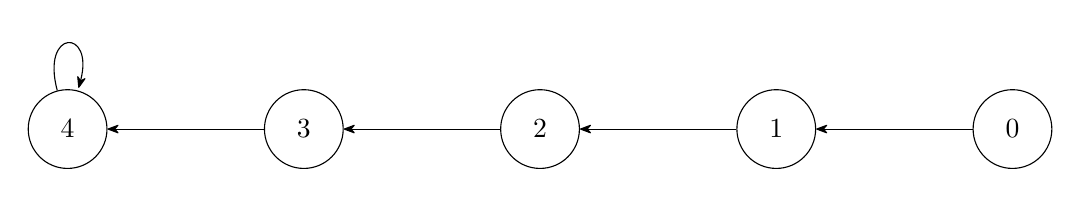
\begin{tikzpicture}[>={Stealth[round]}, node distance=2cm and 1cm, every node/.style={circle, draw, minimum size=1cm}]
    % Define vertices
    \node (v0) at (0, 0) {4};
    \node (v1) at (3, 0) {3};
    \node (v2) at (6, 0) {2};
    \node (v3) at (9, 0) {1};
    \node (v4) at (12, 0) {0};
    
    % Draw edges
    \draw [->] (v1) to (v0); % Edge 1 -> 0
    \draw [->] (v2) to (v1); % Edge 2 -> 1
    \draw [->] (v3) to (v2); % Edge 3 -> 2
    \draw [->] (v4) to (v3); % Edge 4 -> 3
    \draw[->] (v0) edge[loop above] (v0); % Self-loop at 0
\end{tikzpicture}
}
\end{center}
\ \\
\begin{center}   
$G_g: \;$
\resizebox{!}{3em}{
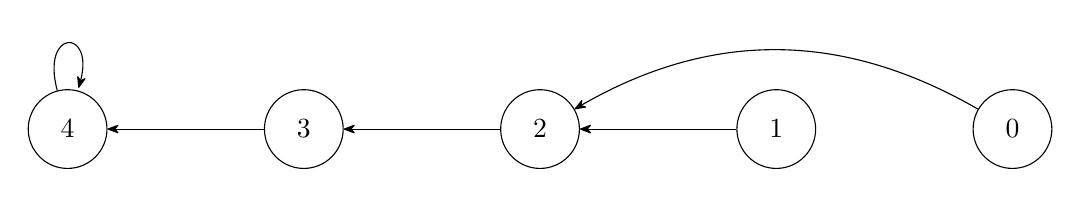
\begin{tikzpicture}[>={Stealth[round]}, node distance=2cm and 1cm, every node/.style={circle, draw, minimum size=1cm}]
    % Define vertices
    \node (v0) at (0, 0) {4};
    \node (v1) at (3, 0) {3};
    \node (v2) at (6, 0) {2};
    \node (v3) at (9, 0) {1};
    \node (v4) at (12, 0) {0};
    
    % Draw edges
    \draw [->] (v1) to (v0); % Edge 1 -> 0
    \draw [->] (v2) to (v1); % Edge 2 -> 1
    \draw [->] (v3) to (v2); % Edge 3 -> 2
    \draw [->] (v4) edge[bend right] (v2); % Edge 4 -> 2
    \draw[->] (v0) edge[loop above] (v0); % Self-loop at 0
\end{tikzpicture}
}
\end{center}
\end{example}


\bibliographystyle{alpha}
\bibliography{biblio}

\end{document}
